%++++++++++++++++++++++++++++++++++++++++
% Don't modify this section unless you know what you're doing!
\documentclass[letterpaper,11pt]{article}
\usepackage{amsmath}
\DeclareMathOperator{\argmax}{\textit{argmax}}
\DeclareMathOperator{\argmin}{arg\,min}
\usepackage{float}
\usepackage{setspace}% http://ctan.org/pkg/setspace
\usepackage[utf8x]{inputenc}
% Inline code utility
\newcommand{\code}[1]{\texttt{#1}}
\usepackage{listings}
\usepackage{color}
\definecolor{light-gray}{gray}{0.95}

\usepackage{algpseudocode}
\usepackage{algorithm}

\usepackage[T1]{fontenc}
\usepackage{inconsolata}
\definecolor{pblue}{rgb}{0.13,0.13,1}
\definecolor{pgreen}{rgb}{0,0.5,0}
\definecolor{pred}{rgb}{0.9,0,0}
\definecolor{pgrey}{rgb}{0.46,0.45,0.48}

\usepackage{listings}
\lstset{language=Python,
  backgroundcolor=\color{light-gray},
  showspaces=false,
  showtabs=false,
  breaklines=true,
  showstringspaces=false,
  breakatwhitespace=true,
  commentstyle=\color{pgreen},
  keywordstyle=\color{pblue},
  stringstyle=\color{pred},
  basicstyle=\fontsize{11}{11}\ttfamily,
  tabsize=4,
  moredelim=[il][\textcolor{pgrey}],
  moredelim=[is][\textcolor{pgrey}]{\%\%}{\%\%},
  frame=tlbr,framesep=4pt,framerule=0pt,
  aboveskip=9pt,
  belowskip=13pt
}

\usepackage{tabularx} % extra features for tabular environment
\usepackage{amsmath}  % improve math presentation
\usepackage{graphicx} % takes care of graphic including machinery
\usepackage[margin=1in,letterpaper]{geometry} % decreases margins
\usepackage{cite} % takes care of citations
\usepackage[final]{hyperref} % adds hyper links inside the generated pdf file
\hypersetup{
	colorlinks=true,       % false: boxed links; true: colored links
	linkcolor=blue,        % color of internal links
	citecolor=blue,        % color of links to bibliography
	filecolor=magenta,     % color of file links
	urlcolor=blue         
}

\usepackage[labelfont=bf]{caption}
\captionsetup{labelfont=bf}
\usepackage[margin=2cm]{caption}

%++++++++++++++++++++++++++++++++++++++++


\begin{document}

\title{Web Information Retrieval}
\author{A student}
\date{March 2019}
\maketitle

\section{Boolean retrieval}

\textbf{Information retrieval} (IR) is finding material (usually documents) of an unstructured nature (usually text) that satisfies an information need from within large collections. The term \textit{unstructured data} refers to data which does not have clear, semantically overt, easy-for-a-computer structure. It is the opposite of structured data, the canonical example of which is a relational database. Almost no data are truly \textit{unstructured}: most text has structure, such as headings and paragraphs and footnotes, which is commonly represented in documents by explicit markup. 

The field of information retrieval also covers supporting users in browsing or filtering document collections or further processing a set of retrieved documents. Given a set of documents, clustering is the task of coming up with a good grouping of the documents based on their contents. Given a set of topics, standing information needs, or other categories (such as suitability of texts for different age groups), classification is the task of deciding which class(es), if any, each of a set of documents belongs to.

Information retrieval systems can also be distinguished by the scale at which they operate, and it is useful to distinguish three prominent scales. In \textbf{web search}, the system has to provide search over billions of documents stored on millions of computers. At the other extreme is \textbf{personal information retrieval}. In the last few years, consumer operating systems have integrated information retrieval (such as Apple's Mac OS X Spotlight). Email programs usually not only provide search but also text classification: they at least provide a spam (junk mail) filter, and commonly also provide either manual or automatic means for classifying mail so that it can be placed directly into particular folders. In between is the space of \textbf{enterprise}, \textbf{institutional}, and \textbf{domain-specific search}, where retrieval might be provided for collections such as a corporation's internal documents.

Our goal is to develop a system to address the \textit{ad hoc} retrieval task. In it, a system aims to provide documents from within the collection that are relevant to an arbitrary user information need. An \textbf{information need} is the topic about which the user desires to know more, and is differentiated from a query, which is what the user conveys to the computer in an attempt to communicate the information need. A document is relevant if it is one that the user perceives as containing information of value with respect to their personal information need. To assess the \textbf{effectiveness} of an IR system (i.e., the quality of its search results), there are two statistics about the system's returned results for a query:
\begin{itemize}
    \item \textbf{Precision}: What fraction of the returned results are relevant to the information need?
    \item \textbf{Recall}: What fraction of the relevant documents in the collection were returned by the system?
\end{itemize}

\subsection{An example information retrieval problem}

Suppose you wanted to determine which plays of Shakespeare contain the words \code{Brutus AND Caesar AND NOT Calpurnia}. One way to do that is to start at the beginning and to read through all the text (grepping through text). But for many purposes, you do need more:
\begin{enumerate}
    \item To process large document collections quickly.
    \item To allow more flexible matching operations. For example, it is impractical to perform the query \code{Romans NEAR countrymen} with grep, where \code{NEAR} might be defined as "within 5 words" or "within the same sentence".
    \item To allow ranked retrieval: in many cases you want the best answer to an information need among many documents that contain certain words.
\end{enumerate}
The way to avoid linearly scanning the texts for each query is to \textbf{index} the documents in advance. Suppose we record for each document whether it contains each word out of all the words Shakespeare used. The result is a binary term-document incidence matrix. Terms are the indexed units; they are usually words. Depending on whether we look at the matrix rows or columns, we can have a vector for each term, which shows the documents it appears in, or a vector for each document, showing the terms that occur in it.
\begin{figure}[H]
    \centering
    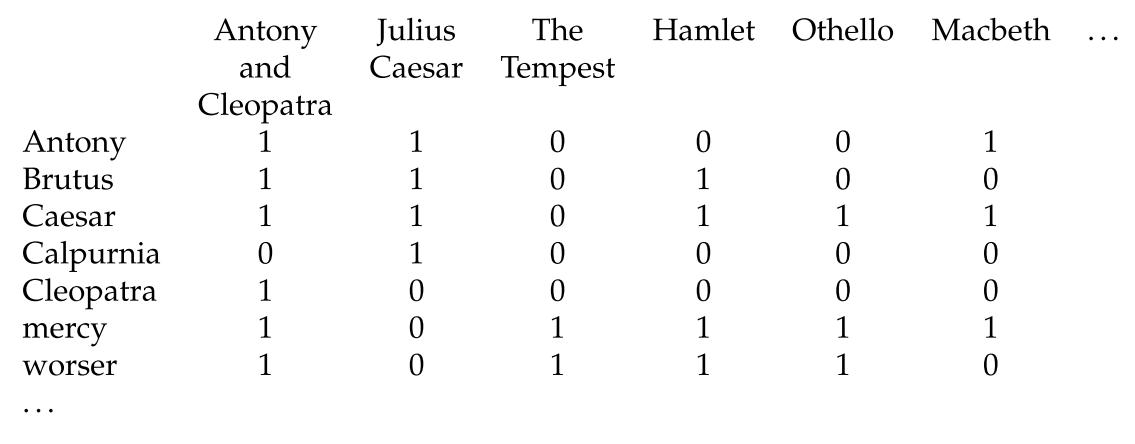
\includegraphics[scale=0.45]{sect1/figure1_1.png}
    \caption{A term-document incidence matrix. Matrix element $(t, d)$ is 1 if the play in column d contains the word in row $t$, and is 0 otherwise.}
\end{figure}
To answer the query \code{Brutus AND Caesar AND NOT Calpurnia}, we take the vectors for Brutus, Caesar and Calpurnia, complement the last, and then do a bitwise \code{AND}:\\
~\\
\centerline{\code{110100 AND 110111 AND 101111 = 100100}}
~\\
The answers for this query are thus \textit{Antony and Cleopatra} and \textit{Hamlet}.

The Boolean retrieval model is a model for information retrieval in which we can pose any query which is in the form of a Boolean expression of terms, that is, in which terms are combined with the operocument as just a set of words.
Suppose we have $N = 1$ million documents. Suppose each document is about 1000 words long. If we assume an average of 6 bytes per word including spaces and punctuation, then this is a document collection about  6 GB in size. Typically, there might be about $M = 500,000$ distinct terms in these documents. A $500K \times 1M$ matrix has half-a-trillion 0's and 1's - too many to fit in a computer's memory. But the matrix is extremely sparse, it has few non-zero entries. Because each document is 1000 words long, the matrix has no more than one billion 1's, so a minimum of $99.8\%$ of the cells are zero.

A much better representation is to record only the 1's occurrences. With \textbf{inverted index} we keep a dictionary of terms. Then for each term, we have a list that records which documents the term occurs in. Each item in the list is called \textbf{posting}, the list is called \textbf{postings list} and all the postings list are called \textbf{postings}.

\subsection{A first take at building an inverted index}

To gain the speed benefits of indexing at retrieval time, we have to build the index in advance. The major steps in this are:
\begin{enumerate}
    \item Collect the documents to be indexed.
    \item Tokenize the text, turning each document into a list of tokens.
    \item Do linguistic preprocessing, producing a list of normalized tokens, which are the indexing terms.
    \item Index the documents that each term occurs in by creating an inverted index, consisting of a dictionary and postings.
\end{enumerate}
\begin{figure}[H]
    \centering
    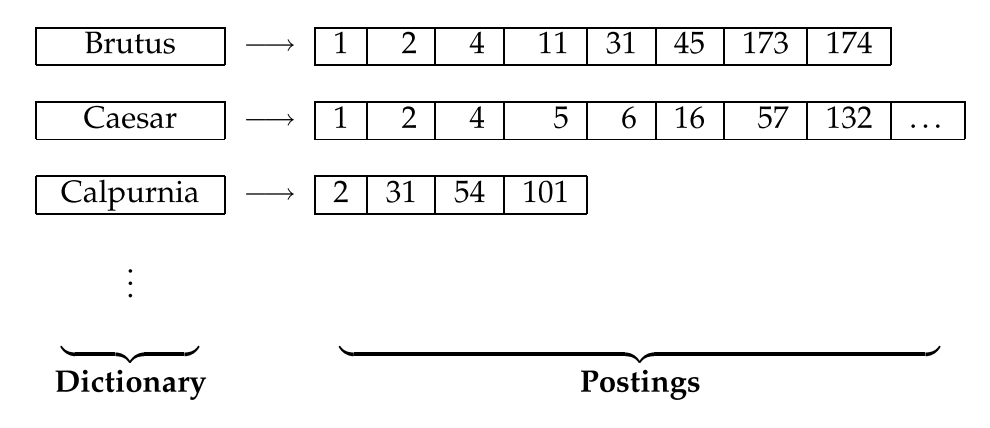
\includegraphics[scale=0.45]{sect1/figure1_3.png}
    \caption{The two parts of an inverted index. The dictionary is kept in memory, with pointers to each postings list, stored on disk.}
\end{figure}
Within a document collection, we assume that each document has a unique serial number, known as the document identifier (\textbf{docID}). The core indexing step is sorting this list so that the terms are alphabetical. Instances of the same term are then grouped, and the result is split into a dictionary and postings. The dictionary also records some statistics, such as the number of documents which contain each term, the \textbf{document frequency}. The postings are secondarily sorted by docID. This provides the basis for efficient query processing. The dictionary is commonly kept in memory, while postings lists are normally kept on disk. What data structure should be used for a postings list? A fixed length array would be wasteful as some words occur in many documents, and others in very few. For an in-memory postings list, two good alternatives are singly linked lists or variable length arrays.

\subsection{Processing Boolean queries}

How do we process a query using an inverted index and the basic Boolean retrieval model? Consider processing the \textit{simple conjunctive query}:\\
~\\
\centerline{\code{Brutus AND Calpurnia}}
~\\
over the inverted index:
\begin{enumerate}
    \item Locate \code{Brutus} in the Dictionary
    \item Retrieve its postings
    \item Locate \code{Calpurnia} in the Dictionary
    \item Retrieve its postings
    \item Intersect the two postings lists
\end{enumerate}
The \textbf{intersection} operation is the crucial one: we need to efficiently intersect postings lists so as to be able to quickly find documents that contain both terms (This operation is sometimes referred to as \textbf{merging} postings lists). There is a simple and effective method of intersecting postings lists using the merge algorithm: we maintain pointers into both lists and walk through the two postings lists simultaneously, in time linear in the total number of postings entries.
\begin{algorithm}[H]
\begin{algorithmic}[1]
\label{INTERSECT} % and a label for \ref{} commands later in the document
\caption{Algorithm for the intersection of two postings lists.}
\Function{INTERSECT}{$p_1$, $p_2$}
    \State $answer \gets \langle \rangle$
    \While {$p_1 \neq NULL$ and $p_2 \neq NULL$}
        \If{$docID(p_1) = docID(p_2)$}
            \State ADD($answer, docID(p_1)$)
            \State $p_1 \gets next(p_2)$
            \State $p_2 \gets next(p_1)$
        \ElsIf{$docID(p_1) < docID(p_2)$}
            \State $p_1 \gets next(p_2)$
            \State $p_2 \gets next(p_1)$
        \EndIf
    \EndWhile
    \State \Return $answer$
\EndFunction
\end{algorithmic}
\end{algorithm}
At each step, we compare the docID pointed to by both pointers. If they are the same, we put that docID in the results list, and advance both pointers. Otherwise we advance the pointer pointing to the smaller docID. If the lengths of the postings lists are $x$ and $y$, the intersection takes $O(x + y)$ operations. To use this algorithm, it is crucial that postings be sorted by a single global ordering.

\textbf{Query optimization} is the process of selecting how to organize the work of answering a query. A major element of this for Boolean queries is the order in which postings lists are accessed. The standard heuristic is to process terms in order of increasing document frequency: if we start by intersecting the two smallest postings lists, then all intermediate results must be no bigger than the smallest postings list.

\subsection{The extended Boolean model versus ranked retrieval}

The Boolean retrieval model contrasts with \textbf{ranked retrieval models} such as the vector space model in which users largely use \textbf{free text queries}, just typing one or more words rather than using a precise language. A strict Boolean expression over terms with an unordered results set is too limited for many of the information needs and most systems implemented extended Boolean retrieval models by incorporating additional operators such as term proximity operators. A \textbf{proximity operator} is a way of specifying that two terms in a query must occur close to each other.

\section{The term vocabulary and postings lists}

The major steps in inverted index construction are:
\begin{enumerate}
    \item Collect the documents to be indexed. 
    \item Tokenize the text.
    \item Do linguistic preprocessing of tokens.
    \item Index the documents that each term occurs in.
\end{enumerate}
\textbf{Tokenization} is the process of chopping character streams into tokens, while linguistic preprocessing then deals with building equivalence classes of tokens which are the set of terms that are indexed.

\subsection{Document delineation and character sequence decoding}

\paragraph{Obtaining the character sequence in a document}
Digital documents that are the input to an indexing process are typically bytes in a file or on a web server. The first step of processing is to convert this byte sequence into a linear sequence of characters, by determining the correct encoding. This can be regarded as a machine learning classification problem. Once the encoding is determined, we decode the byte sequence to a character sequence. 

The characters may have to be decoded out of some binary representation like Microsoft Word DOC files and/or a compressed format such as zip files. Even for plain text documents, additional decoding may need to be done. In XML documents, character entities, such as \code{\&amp;} (\&), need to be decoded to give the correct character. Finally, the textual part of the document may need to be extracted out of other material that will not be processed.

\paragraph{Choosing a document unit}
The next phase is to determine what the \textbf{document unit} for indexing is. For a collection of books, it would usually be a bad idea to index an entire book as a document. Instead, we may well wish to index each chapter or paragraph as a mini-document. Matches are thenmore likely to be relevant, and since the documents are smaller it will be much easier for the user to find the relevant passages in the document. We could treat individual sentences as mini-documents. But, if the units get too small, we are likely to miss important passages because terms were distributed over several mini-documents, while if units are too large we tend to get spurious matches and the relevant information is hard for the user to find. The issue of \textbf{indexing granularity} is responsible of a precision/recall trade-off.

\subsection{Determining the vocabulary of terms}

\paragraph{Tokenization}
Given a character sequence and a defined document unit, tokenization is the task of chopping it up into pieces, called \textbf{tokens}, throwing away certain characters, such as punctuation.
\begin{figure}[H]
    \centering
    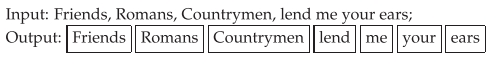
\includegraphics[scale=0.8]{sect2/figure2_1.png}
    \caption{Example of tokenization.}
\end{figure}
A \textbf{token} is an instance of a sequence of characters in some particular document that are grouped together as a semantic unit for processing. A \textbf{type} is the class of all tokens containing the same character sequence. A \textbf{term} is a type that is included in the IR system’s dictionary.

The major question of the tokenization phase is what are the correct tokens to use? For example, what do you do about the various uses of the apostrophe? For the text \textit{Finland's capital} which is the best tokenization? \code{Finland} \code{AND} \code{s}, \code{Finlands} or \code{Finland's}? 

These issues of tokenization are language-specific. It thus requires the language of the document to be known. \textbf{Language identification} based on classifiers that use short character subsequences as features is highly effective; most languages have distinctive signature patterns.

In English, \textbf{hyphenation} is used for various purposes ranging from splitting up vowels in words, \textit{co-education}, to joining nouns as names, \textit{Hewlett-Packard}, to a copy editing device to show word grouping, \textit{the hold-him-backand-drag-him-away maneuver}. Handling hyphens automatically can be complex: it can either be done as a classification problem, or more commonly by some heuristic rules, such as allowing short hyphenated prefixes on words, but not longer hyphenated forms. 

Splitting on white space can also split what should be regarded as a single token. This occurs most commonly with names, \textit{San Francisco}, but also with borrowed foreign phrases, \textit{au fait}, and compounds that are sometimes written as a single word and sometimes space separated (such as \textit{white space} vs. \textit{whitespace}).

One effective strategy in practice, which is used by some Boolean retrieval systems is to encourage users to enter hyphens wherever they may be possible, and whenever there is a hyphenated form, the system will generalize the query to cover all three of the one word, hyphenated, and two word forms. However, this strategy depends on user training.

\paragraph{Dropping common terms: stop words}
Sometimes, some extremely common words which would appear to be of little value. These words are called \textbf{stop words}. The general strategy for determining a stop list is to sort the terms by \textbf{collection frequency} (the total number of times each term appears in the document collection) and then to take the most frequent terms, often hand-filtered for their semantic content relative to the domain of the documents being indexed, as a stop list, the members of which are then discarded during indexing. Using a stop list significantly reduces the number of postings that a system has to store. And a lot of the time not indexing stop words does little harm: keyword searches with terms like the and by don't seem very useful. However, this is not true every time. For example, the meaning of \textit{flights to London} is likely to be lost if the word \code{to} is stopped out.

The general trend in IR systems over time has been from standard use of quite large stop lists (200-300 terms) to very small stop lists (7-12 terms) to no stop list. Web search engines generally do not use stop lists. Some of the design of modern IR systems has focused precisely on how we can exploit the statistics of language so as to be able to cope with common words in better ways. For most modern IR systems, the additional cost of including stop words is not that big – neither in terms of index size nor in terms of query processing time.

\paragraph{Normalization (equivalence classing of terms)}
The easy case is if tokens in the query just match tokens in the token list of the document. However, there are many cases when two character sequences are not quite the same but you would like a match to occur.

\textbf{Token normalization} is the process of canonicalizing tokens so that matches occur despite superficial differences in the character sequences of the tokens. The most standard way to normalize is to implicitly create \textbf{equivalence classes}. For instance, if the tokens \textit{anti-discriminatory} and \textit{antidiscriminatory} are both mapped onto the term \code{antidiscriminatory}, in both the document text and queries, then searches for one term will retrieve documents that contain either.

An alternative to creating equivalence classes is to maintain relations betweenunnormalized tokens. Thismethod can be extended to hand-constructed lists of synonyms such as \textit{car} and \textit{automobile}. These term relationships can be achieved in two ways. The usual way is to index unnormalized tokens and to maintain a query expansion list of multiple vocabulary entries to consider for a certain query term. A query term becomes a disjunction of several postings lists. The alternative is to perform the expansion during index construction. The alternative is to perform the expansion during index construction. When the document contains automobile, we index it under car as well, and, usually, also vice-versa. Use of either of these methods is considerably less efficient than equivalence classing.

These are some forms of normalization that are commonly used:
\begin{itemize}
    \item \textbf{Accents and diacritics.} Diacritics on characters in English have a fairly marginal status, and we might well want \textit{cliché} and \textit{cliche} to match, or \textit{naive} and \textit{naïve}. This can be done by normalizing tokens to remove diacritics. In many other languages, diacritics are a regular part of the writing system and distinguish different sounds. 
    \item \textbf{Capitalization/case-folding.} A common strategy is to do case-folding by reducing all letters to lower case.It will allow instances of \textit{Automobile} at the beginning of a sentence to match with a query of \textit{automobile}. It will also help on a web search engine when most of your users type in \textit{ferrari} when they are interested in a \textit{Ferrari} car. On the other hand, such case folding can equate words that might better be kept apart. Many proper nouns are derived from common nouns and so are distinguished only by case, including companies, government organizations and person names. For English, the simplest heuristic is to convert to lowercase words at the beginning of a sentence. Mid-sentence capitalized words are left as capitalized. This is known as \textbf{truecasing}.
    \item \textbf{Other issues in English.} For instance, you might wish to equate \textit{ne’er} and \textit{never} or the British spelling \textit{colour} and the American spelling \textit{color}. Dates, times and similar items come in multiple formats, presenting additional challenges. You might wish to collapse together \textit{3/12/91} and \textit{Mar. 12, 1991}.
    \item \textbf{Other languages.} Other languages present distinctive issues in equivalence classing. The French word for \textit{the} has distinctive forms based not only on the gender (masculine or feminine) and number of the following noun, but also depending on whether the following word begins with a vowel. We may well wish to equivalence class these various forms of the. German has a convention whereby vowels with an umlaut can be rendered instead as a two vowel digraph. We would want to treat \textit{Schütze} and \textit{Schuetze} as equivalent. Document collections being indexed can include documents from many different languages. Or a single document can easily contain text from multiple languages. Most commonly, the language is detected and language-particular tokenization and normalization rules are applied at a predetermined granularity.
\end{itemize}

\paragraph{Stemming and lemmatization}
For grammatical reasons, documents are going to use different forms of a word, such as \textit{organize}, \textit{organizes}, and \textit{organizing}. Additionally, there are families of related words with similar meanings, such as \textit{democracy}, \textit{democratic}, and \textit{democratization}. It's useful for a search for one of these words to return documents that contain another word in the set.\\
The goal of both stemming and lemmatization is to reduce inflectional forms, for instance:
\medskip\\
\indent am, are, is $\Rightarrow$ be\\
\indent car, cars, car’s, cars’ $\Rightarrow$ car
\medskip\\
\textbf{Stemming} usually refers to a heuristic process that chops off the ends of words in the hope of achieving this goal correctly most of the time, includes the removal of derivational affixes. \textbf{Lemmatization} usually refers to doing things properly with the use of a vocabulary and morphological analysis of words, normally aiming to remove inflectional endings only and to return the base or dictionary form of a word, which is known as the \textbf{lemma}. For example, the token \textit{saw}, stemming might return just \textit{s}, whereas lemmatization would attempt to return either \textit{see} or \textit{saw}.

The most common algorithm for stemming English is \textit{Porter’s algorithm}. Porter’s algorithm consists of 5 phases of word reductions, applied sequentially. Within each phase there are various conventions to select rules (sample convention: \textit{Of the rules in a compound command, select the one that applies to the longest suffix}). Some typical rules are:
\begin{itemize}
    \item Substitution
    \begin{itemize}
        \item SSES $\rightarrow$ SS
        \item IES $\rightarrow$ I
        \item SS $\rightarrow$ SS
        \item S $\rightarrow$ 
    \end{itemize}
    \item Weight of word sensitive rules
    \item ($m > 1$) EMENT $\rightarrow$
    \begin{itemize}
        \item \textit{replacement} $\rightarrow$ \textit{replac}
        \item \textit{cement} $\rightarrow$ \textit{cement}
    \end{itemize}
\end{itemize}
Stemmers use language-specific rules, but they require less knowledge than a lemmatizer, which needs a complete vocabulary and morphological analysis to correctly lemmatize words.

A \textbf{lemmatizer} is a tool from Natural Language Processing which does full morphological analysis to accurately identify the lemma for each word. Doing full morphological analysis produces at most very modest benefits for retrieval. While it helps a lot for some queries, it equally hurts performance a lot for others. Stemming increases recall while harming precision. For example, the Porter stemmer stems all of the following words:
\medskip\\
\indent \textit{operate operating operates operation operative operatives operational}
\medskip\\
to \textit{oper}. However, since operate in its various forms is a common verb, we would expect to lose precision on queries such as:
\medskip\\
\indent \textit{operative} (\textit{dentistry}) $\Rightarrow$ \textit{oper}
\medskip\\
The situation is different for languages with much more morphology, such
as Spanish, German, and Finnish.

\subsection{Faster postings list intersection via skip pointers}
In the basic postings list intersection, ff the list lengths are $m$ and $n$, the intersection takes $O(m+ n)$ operations. One way to do better than this is to use a \textbf{skip list} by augmenting postings lists with skip pointers (at indexing time). Skip pointers allow us to avoid processing parts of the postings list that will not figure in the search results.
\begin{figure}[H]
    \centering
    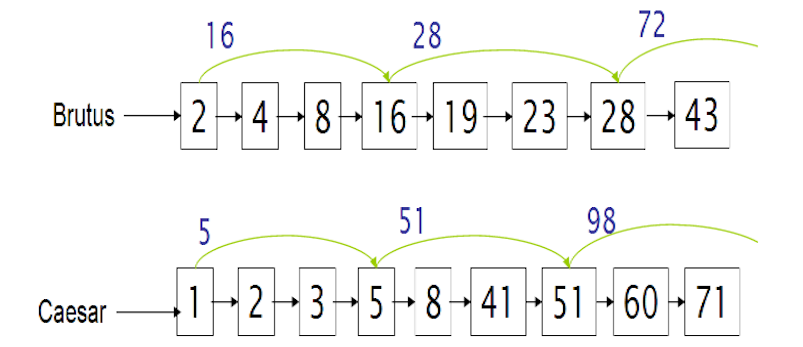
\includegraphics[scale=0.65]{sect2/figure_2_9.png}
    \caption{Postings lists with skip pointers.}
\end{figure}
 Where do we place skips? There is a trade-off. More skips means shorter
skip spans, and we are more likely to skip. But it also means lots of comparisons to skip pointers, and lots of space storing skip pointers. Fewer skips means few pointer comparisons, but then long skip spans which means that there will be fewer opportunities to skip. A simple heuristic is that for a postings list of length $P$, use $\sqrt{P}$ evenly-spaced skip pointers. Building effective skip pointers is easy if an index is relatively static; it
is harder if a postings list keeps changing because of updates.

\subsection{Positional postings and phrase queries}
Most recent search engines support a double quotes syntax (\textit{stanford university}) for \textbf{phrase queries}, which has proven to be very easily understood and successfully used by users. To be able to support such queries, it is no longer sufficient for postings lists to be simply lists of documents that contain individual terms. There are two approaches.

\paragraph{Biword indexes}
One approach is to consider every pair of consecutive terms in a document as a phrase. For example, the text \textit{Friends}, \textit{Romans}, \textit{Countrymen} would generate the \textbf{biwords}:
\medskip\\
\indent \code{friends romans}\\
\indent \code{romans countrymen}
\medskip\\
We treat each of these biwords as a vocabulary term. First, we tokenize the text and perform part-of-speech-tagging. We can then group terms into nouns, including proper nouns, (N) and function words, including articles and prepositions, (X), among other classes. Any string of terms of the form $NX*N$ is an extended biword. Each such extended biword is made a term in the vocabulary. To process a query using such an extended biword index, we need to also parse it into N’s and X’s, and then segment the query into extended biwords.

This algorithm does not always work in an intuitively optimal manner when parsing longer queries into Boolean queries. Using the above algorithm, the query
\medskip\\
\indent \code{cost overruns on a power plant}
\medskip\\
is parsed into
\medskip\\
\indent \code{“cost overruns” AND “overruns power” AND “power plant”}
\medskip\\
whereas it might seem a better query to omit the middle biword.

Searches for a single term are not naturally handled in a biword index, and so we also need to have an index of single-word terms. But storing longer phrases has the potential to greatly expand the vocabulary size.

\paragraph{Positional indexes}
A biword index is not the standard solution, a \textbf{positional index} is most commonly employed. Here, for each term in the vocabulary, we store postings of the form docID: $\langle position1, position2, \dots \rangle$ where each position is a token index in the document. Each posting will also usually record the term frequency. 

To process a phrase query, you still need to access the inverted index. As before, you would start with the least frequent term and then restrict the list of possible candidates. In the merge operation, the same general technique is used as before, but you also need to check that their positions of appearance in the document are compatible with the phrase query being evaluated. The same general method is applied for within $k$ word proximity searches:
\medskip\\
\code{employment /3 place}
\medskip\\
$/k$ means "within k words of". Positional indexes can be used for such queries; biword indexes cannot.

Adopting a positional index expands required postings storage significantly. Moving to a positional index also changes the asymptotic complexity of a postings intersection operation, because the number of items to check is now bounded not by the number of documents but by the total number of tokens in the document collection $T$: the complexity of a Boolean query is $\Theta(T)$ rather than $\Theta(N)$.

\paragraph{Combination schemes}
The strategies of biword indexes and positional indexes can be fruitfully combined. If users commonly query on particular phrases, such as \code{Michael Jackson}, it is quite inefficient to keep merging positional postings lists. A combination strategy uses a phrase index, or just a biword index, for certain queries and uses a positional index for other phrase queries.

\section{Dictionaries and tolerant retrieval}
We will discuss techniques that are robust to typographical errors in the query, as well as alternative spellings. A \textbf{wildcard query} $^*$ symbol indicates any (possibly empty) string of characters: a query such as \code{*a*e*i*o*u*}, which seeks documents containing any term that includes all the five vowels in sequence.

\subsection{Search structures for dictionaries}
Given an inverted index and a query, our first task is to determine whether each query term exists in the vocabulary and if so, identify the pointer to the corresponding postings. This vocabulary lookup operation uses a classical data structure called the dictionary (hashing or search trees).

\textbf{Hashing} has been used for dictionary lookup in some search engines. Each
vocabulary term (\textbf{key}) is hashed into an integer over a large enough space that hash collisions are unlikely. At query time, we hash each query term separately and following a pointer to the corresponding postings. There is no easy way to find minor variants of a query term since these could be hashed to very different integers. In a setting (such as the Web) where the size of the vocabulary keeps growing, a hash function designed for current needs may not scale well.

\textbf{Search trees} overcome many of these issues. The best-known search tree is the \textbf{binary tree}: the search for a term begins at the root of the tree. Each internal node (including the root) represents a binary test. Efficient search (with a number of comparisons that is $O(\log M)$) hinges on the tree being balanced: the numbers of terms under the two sub-trees of any node are either equal or differ by one. The principal issue here is that of rebalancing: as terms are inserted into or deleted from the binary search tree, it needs to be rebalanced so that the balance property is maintained.

To mitigate rebalancing, one approach is to allow the number of sub-trees under an internal node to vary in a fixed interval. A search tree commonly used is the \textbf{B-tree}, in which every internal node
has a number of children in the interval $[a, b]$, where $a$ and $b$ are positive integers.
\begin{figure}[H]
    \centering
    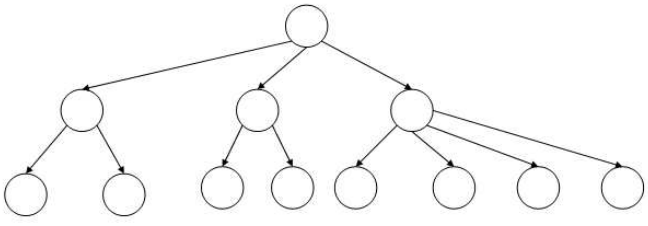
\includegraphics[scale=0.55]{sect3/figure_3_2.png}
    \caption{A B-tree. In this example every internal node has between 2 and 4 children.}
\end{figure}
Unlike hashing, search trees demand that the characters used in the document collection have a prescribed ordering.

\subsection{Wildcard queries}
Wildcard queries are used in any of the following situations: (1) the user is uncertain of the spelling of a query term (e.g., \code{Sydney} vs. \code{Sidney}, which leads to the wildcard query \code{S*dney}); (2) the user is aware of multiple variants of spelling a term and (consciously) seeks documents containing any of the variants (e.g., \code{color} vs. \code{colour}); (3) the user seeks documents containing variants of a term that would be caught by stemming, but is unsure whether the search engine performs stemming stemming (e.g., \code{judicial} vs. \code{judiciary}, the wildcard query \code{judicia*}); (4) the user is uncertain of the correct rendition of a foreign word or phrase (e.g., the query \code{Universit* Stuttgart}).

A query such as \code{mon*} is known as a \textbf{trailing wildcard query}, because the $^*$ symbol occurs only once, at the end of the search string. We walk down the tree following the symbols \code{m}, \code{o} and \code{n} in turn, for each we can enumerate the set $W$ of terms in the dictionary with the prefix \code{mon}. Finally, we use $|W|$ lookups on the standard inverted index to retrieve all documents containing any term in $W$. 

Consider now \textbf{leading wildcard queries}, queries of the form \code{*mon}. Consider a \textbf{reverse B-tree} on the dictionary, one in which each root-to-leaf path of the B-tree corresponds to a term in the dictionary written \textbf{backwards}: the term \code{lemon} would, in the B-tree, be represented by the path \code{root-n-o-m-e-l}.

Using a regular B-tree together with a reverse B-tree, we can handle an even more general case: wildcard queries in which there is a single $^*$ symbol, such as \code{se*mon}.The regular B-tree is used to enumerate the set $W$ of dictionary terms beginning with the prefix \code{se}, then the reverse B-tree to enumerate the set $R$ of terms ending with the suffix \code{mon}. Next, we take the intersection $W \cap R$ of these two sets. Finally, we use the standard inverted index to retrieve all documents containing any terms in this intersection.

\paragraph{General wildcard queries}
There are two techniques for handling general wildcard queries. Both techniques share a common strategy: express the given wildcard query $q_w$ as a Boolean query $Q$ on a specially constructed index, such that the answer to $Q$ is a superset of the set of vocabulary terms matching $q_w$. Then, we check each term in the answer to $Q$ against $q_w$, discarding those vocabulary terms that do not match $q_w$.

The first special index for general wildcard queries is the \textbf{permuterm index}, a form of inverted index. First, we introduce a special symbol \$, used to mark the end of a term. The term \code{hello} is shown here as the augmented term \code{hello\$}. Next, we construct a permuterm index, in which the various rotations of each term (augmented with \$) all link to the original vocabulary term. The set of rotated terms in the permuterm index is the permuterm vocabulary.

Consider the wildcard query \code{m*n}. The key is to rotate such a wildcard query so that the $^*$ symbol appears at the end of the string, \code{n\$m*}. Next, we look up this string in the permuterm index, where seeking \code{n\$m*} (via a search tree) leads to rotations of (among others) the terms \code{man} and \code{moron}. Now we look up these terms in the standard inverted index to retrieve matching documents. We can thus handle any wildcard query with a single $^*$ symbol. In query such as \code{fi*mo*er}, we first enumerate the terms in the dictionary that are in the permuterm index of \code{er\$fi*}, then we filter out the entries that don't contain \code{mo}. One disadvantage of the permuterm index is that its dictionary becomes quite large.
\begin{figure}[H]
    \centering
    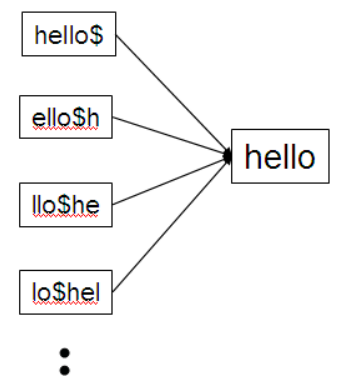
\includegraphics[scale=0.55]{sect3/figure_3_3.png}
    \caption{A portion of a permuterm index.}
\end{figure}

\paragraph{$k$-gram indexes for wildcard queries}
A \textbf{$k$-gram} is a sequence of $k$ characters. For example \code{cas}, \code{ast} and \code{stl} are all 3-grams occurring in the term \code{castle}. A special character \$ is used to denote the beginning or end of a term, so the full set of 3-grams generated for \code{castle} is: \code{\$ca}, \code{cas}, \code{ast}, \code{stl}, \code{tle}, \code{le\$}.

In a $k$-gram index, the dictionary contains all $k$-grams that occur in any term in the vocabulary. Each postings list points from a $k$-gram to all vocabulary terms containing that $k$-gram. For instance, the 3-gram \code{etr} would point to vocabulary terms such as \code{metric} and \code{retrieval}.
\begin{figure}[H]
    \centering
    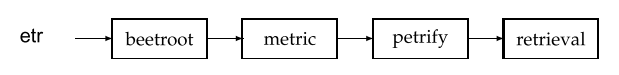
\includegraphics[scale=0.70]{sect3/figure_3_4.png}
    \caption{Example of a postings list in a 3-gram index.}
\end{figure}

There is a difficulty with the use of $k$-gram indexes, that demands one further step of processing. Consider the query \code{red*}. We first issue the Boolean query \code{\$re AND red} to the 3-gram index. This leads to a match on terms such as \code{retired}, which contain the conjunction of the two 3grams \code{\$re} and \code{red}, yet do not match the original wildcard query \code{red*}. To handle this, we introduce a \textbf{post-filtering} step, in which the terms enumerated by the Boolean query on the 3-gram index are checked individually against the original query. Terms that survive are then searched in the standard inverted index.

The processing of a wildcard query can be quite expensive because of the added lookup in the special index, filtering and finally the standard inverted index. A search engine may support such rich functionality, but most commonly, the capability is hidden behind an interface that most users never use.

\subsection{Spelling correction}
There are two methods to solve the problem of correcting spelling errors in queries: the first based on \textbf{edit distance} and the second based on \textbf{$k$-gram overlap}.

\paragraph{Implementing spelling correction}
There are two basic principles underlying most spelling correction algorithms.
\begin{enumerate}
    \item Of various alternative correct spellings for a mis-spelled query, choose the “nearest” one.
    \item When two correctly spelled queries are tied (or nearly tied), select the one that is more common.
\end{enumerate}

Spelling correction algorithms are exposed to users in one of several ways:
\begin{enumerate}
    \item On the query \code{carot} always retrieve documents containing \code{carot} as well as any “spell-corrected” version of \code{carot}, including \code{carrot} and \code{tarot}.
    \item As in (1) above, but only when the query term \code{carot} is not in the dictionary.
    \item As in (1) above, but only when the original query returned fewer than a preset number of documents.
    \item When the original query returns fewer than a preset number of documents, the search interface presents a spelling suggestion to the end user: “Did you mean carrot?”
\end{enumerate}

\paragraph{Forms of spelling correction}
We focus on two specific forms of spelling correction, \textbf{isolated-term correction} and \textbf{context-sensitive correction}. In isolated-term correction, we attempt to correct a single query term at a time. Such isolated-term correction would fail to detect, for instance, that the query \code{flew form Heathrow} contains a mis-spelling of the term \code{from}, because each term in the query is correctly spelled in isolation.

\paragraph{Edit distance}
Given two character strings $s_1$ and $s_2$, the \textbf{edit distance} between them is the minimum number of edit operations required to transform $s_1$ into $s_2$. The edit operations allowed for this purpose are: (i) insert a character into a string; (ii) delete a character from a string and (iii) replace a character of a string by another character; edit distance is known as \textbf{Levenshtein distance}. For example, the edit distance between \code{cat} and \code{dog} is 3.

To compute the (weighted) edit distance between two strings in time $O(|s_1|\times|s_2|)$, where $|s_i|$ denotes the length of a string $s_i$. The idea is to use the dynamic programming.

The spelling correction problem however demands more than computing edit distance: given a set $S$ of strings and a query string $q$, we seek the $string(s)$ in $V$ of least edit distance from $q$. The obvious way of doing this is to compute the edit distance from $q$ to each string in $V$, before selecting the $string(s)$ of minimum edit distance. This exhaustive search is expensive.

The simplest heuristic is to restrict the search to dictionary terms beginning with the same letter as the query string. A more sophisticated variant of this heuristic is to use a version of the permuterm index.

\paragraph{$k$-gram indexes for spelling correction}
To further limit the set of vocabulary terms for which we compute edit distances to the query term we can use the $k$-gram index to assist with retrieving vocabulary terms with low edit distance to the query $q$. We will use the $k$-gram index to retrieve vocabulary terms that have many $k$-grams in common with the query. The retrieval process is essentially that of a single scan through the postings for the $k$-grams in the query string $q$.
\begin{figure}[H]
    \centering
    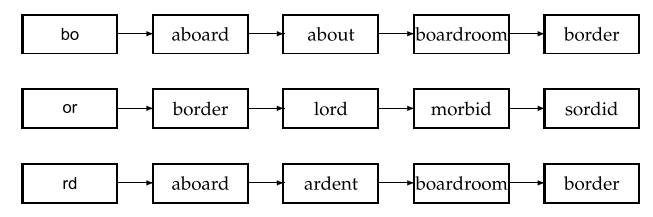
\includegraphics[scale=0.70]{sect3/figure_3_7.png}
    \caption{Matching at least two of the three 2-grams in the query \code{bord}.}
\end{figure}

The linear scan intersection can be adapted when the measure of overlap is the \textbf{Jaccard coefficient} for measuring the overlap between two sets $A$ and $B$, defined to be $|A \cup B|/|A \cup B|$. The two sets we consider are the set of $k$-grams in the query q, and the set of $k$-grams in a vocabulary term. The scan proceeds from one vocabulary term $t$ to the next, computing on the fly the Jaccard coefficient between $q$ and $t$. If the coefficient exceeds a preset threshold, we add $t$ to the output; if not, we move on to the next term in the postings. To compute the Jaccard coefficient, we only need the length of the string $t$.

We could replace the Jaccard coefficient by other measures that allow efficient on the fly computation during postings scans. We can use the $k$-gram index to enumerate a set of candidate vocabulary terms that are potential corrections of $q$. We then compute the edit distance from $q$ to each term in this set, selecting terms from the set with small edit distance to $q$.

\paragraph{Context sensitive spelling correction}
Isolated-term correction would fail to correct typographical errors where all query terms are correctly spelled. The simplest way to correct these errors is to enumerate corrections of each of the query terms even though each query term is correctly spelled, then try substitutions of each correction in the phrase. For the example \code{flew form Heathrow}, we enumerate such phrases as \code{fled form Heathrow} and \code{flew fore Heathrow}. For each such substitute phrase, the search engine runs the query and determines the number of matching results. This enumeration can be expensive, several heuristics are used to reduce the search space.
 
\subsection{Phonetic correction}
\textbf{Phonetic correction}: misspellings that arise because the user types a query that sounds like the target term. Such algorithms are especially applicable to searches on the names of people. The main idea here is to generate, for each term, a \textbf{phonetic hash} so that similar-sounding terms hash to the same value.

Algorithms for such phonetic hashing are commonly collectively known as \textbf{soundex} algorithms. The common steps are:
\begin{enumerate}
    \item Turn every term to be indexed into a 4-character reduced form. Build an inverted index from these reduced forms to the original terms; call this the soundex index.
    \item Do the same with query terms.
    \item When the query calls for a soundex match, search this soundex index.
\end{enumerate}
A commonly used conversion results in a 4-character code, with the first character being a letter of the alphabet and the other three being digits between 0 and 9.
\begin{enumerate}
    \item Retain the first letter of the term.
    \item Change all occurrences of the following letters to ’0’ (zero): ’A’, E’, ’I’, ’O’,
’U’, ’H’, ’W’, ’Y’.
    \item Change letters to digits as follows: \\ 
    \indent B, F, P, V to 1.\\ 
    \indent C, G, J, K, Q, S, X, Z to 2.\\ 
    \indent D,T to 3.\\ 
    \indent L to 4.\\ 
    \indent M, N to 5.\\
    \indent R to 6.
    \item Repeatedly remove one out of each pair of consecutive identical digits.
    \item Remove all zeros from the resulting string. Pad the resulting string with trailing zeros and return the first four positions, which will consist of a letter followed by three digits.
\end{enumerate}
This algorithm rests on a few observations: (1) vowels are viewed as interchangeable, in transcribing names; (2) consonants with similar sounds are put in equivalence classes.

\section{Index construction}
The construction process of an inverted index is called \textbf{index construction} or \textbf{indexing}; the process or machine that performs it the \textbf{indexer}.

\subsection{Hardware basics}
When building an information retrieval (IR) system, many decisions are based on the characteristics of the computer hardware. There are some considerations:
\begin{itemize}
    \item Access to data in memory is much faster than access to data on disk, so we want to keep as much data as possible in memory. The technique of keeping frequently used disk data in main memory \textbf{caching}.
    \item When doing a disk read or write, it takes a while for the disk head to move to the part of the disk where the data are located. This time is called the \textbf{seek time}. No data are being transferred during the seek. To maximize data transfer rates, chunks of data that will be read together should therefore be stored contiguously on disk.
    \item Operating systems generally read and write entire blocks. Thus, reading a single byte from disk can take as much time as reading the entire block.
    \item Data transfers from disk to memory are handled by the system bus, not by the processor. This means that the processor is available to process data during disk I/O. We can speed up data transfers by storing compressed data on disk.
\end{itemize}

\subsection{Blocked sort-based indexing}
First, we introduce the basic steps in constructing a nonpositional index. We first make a pass through the collection assembling all term–docID pairs. We then sort the pairs with the term as the dominant key and docID as the secondary key. Finally, we organize the docIDs for each term into a postings list and compute statistics like term and document frequency. For small collections, all this can be done in memory.

To make index construction more efficient, we represent terms as termIDs, where each \textbf{termID} is a unique. We can build the mapping from terms to termIDs on the fly while we are processing the collection; or, in a two-pass approach, we compile the vocabulary in the first pass and construct the inverted index in the second pass.

We work with the \textit{Reuters-RCV1} collection as our model collection with roughly 1 GB of text. It consists of about 800,000 documents. Reuters-RCV1 has 100million tokens. Collecting all termID–docID pairs of
the collection using 4 bytes each for termID and docID therefore requires 0.8 GB of storage.

With main memory insufficient, we need to use an\textbf{ external sorting algorithm}. For acceptable speed, the central requirement of such an algorithm is that it minimize the number of random disk seeks during sorting. One solution is the \textbf{blocked sort-based indexing algorithm} or \textbf{BSBI}. BSBI (i) segments the collection into parts of equal size, (ii) sorts the termID–docID pairs of each part in memory, (iii) stores intermediate sorted results on disk, and (iv) merges all intermediate results into the final index.

The algorithm parses documents into termID–docID pairs and accumulates the pairs in memory until a block of a fixed size is full. The block is then inverted and written to disk. \textbf{Inversion} involves two steps. First, we sort the termID–docID pairs. Next, we collect all termID–docID pairs with the same termID into a postings list, where a \textbf{posting} is simply a docID. The result is then written to disk. In the final step, the algorithm simultaneously merges the ten blocks into one large merged index.
\begin{algorithm}[H]
\begin{algorithmic}[1]
\label{BSBINDEXCONSTRUCTION} % and a label for \ref{} commands later in the document
\caption{Blocked sort-based indexing. The algorithm stores inverted blocks in files $f_1,\dots, f_n$ and the merged index in $f_{merged}$.}
\Function{BSBI\_CONSTRUCTION}{}
    \State $n \gets 0$
    \While {all documents have not been processed}
        \State $n \gets n + 1$
        \State $block \gets PARSE\_NEXT\_BLOCK()$
        \State $BSBI\_INVERT(block)$
        \State $WRITE\_BLOCK_TO\_DISK(block,f_n)$
    \EndWhile
    \State $MERGE\_BLOCKS(f_1, \dots, f_n, f_{merged})$
\EndFunction
\end{algorithmic}
\end{algorithm}

How expensive is BSBI? Its time complexity is $\Theta(T\log T)$ because the step with the highest time complexity is sorting and $T$ is an upper bound for the number of items we must sort. But the actual indexing time is usually dominated by the time it takes to parse the documents (\code{ PARSE\_NEXT\_BLOCK}) and to do the final merge (\code{MERGE\_BLOCKS}).

\subsection{Single-pass in-memory indexing}
Blocked sort-based indexing has excellent scaling properties, but it needs a data structure for mapping terms to termIDs. For very large collections, this data structure does not fit into memory. A more scalable alternative is \textbf{single-pass in-memory indexing} or \textbf{SPIMI}. SPIMI uses terms instead of termIDs, writes each block’s dictionary to disk, and then starts a new dictionary for the next block. \code{SPIMI\_INVERT} is called repeatedly on the token stream until the entire collection has been processed. Tokens are processed one by one during each successive call of \code{SPIMI\_INVERT}. When a term occurs for the first time, it is added to the dictionary, and a new postings list is created. At the end it returns this postings list for subsequent occurrences of the term.

A difference between BSBI and SPIMI is that SPIMI adds a posting directly to its postings list. Instead of first collecting all termID–docID pairs and then sorting them, each postings list is dynamic and it is immediately available to collect postings. This has two advantages: it is faster because there is no sorting, and it saves memory because we keep track of the term a postings list belongs to, so the termIDs of postings need not be stored.

Because we do not know how large the postings list of a term will be when we first encounter it, we allocate space for a short postings list initially and double the space each time it is full.

When memory has been exhausted, we write the index of the block to disk. We have to sort the terms before doing this because we want to write postings lists in lexicographic order to facilitate the final merging step. If each block’s postings lists were written in unsorted order, merging blocks could not be accomplished by a simple linear scan.

Each call of \code{SPIMI\_INVERT} writes a block to disk, just as in BSBI. The last step of SPIMI is then to merge the blocks into the final inverted index.

SPIMI has a third important component: compression. Both the postings and the dictionary terms can be stored compactly on disk.

The time complexity of SPIMI is $\Theta(T)$ because no sorting of tokens is required and all operations are at most linear in the size of the collection.

\begin{algorithm}[H] 
\begin{algorithmic}[1]
\label{SPIMI_INVERT} % and a label for \ref{} commands later in the document
\caption{Inversion of a block in single-pass in-memory indexing.}
\Function{SPIMI\_INVERT}{$token\_stream$}
    \State $output_file = NEW\_FILE()$
    \State $dictionary = NEW\_HASH()$
    \While {free memory available}
        \State $token \gets next(token\_stream)$
         \If{$term(token) \notin dictionary$}
            \State $postings\_list =$ ADD\_TO\_DICTIONARY$(dictionary, term(token))$
        \Else
            \State $postings\_list =$ GET\_POSTINGS\_LIST$(dictionary, term(token))$
            \State $p_2 \gets next(p_1)$
        \EndIf
        \If{$full(postings\_list)$}
            \State $postings\_list =$ DOUBLE\_POSTINGS\_LIST$(dictionary, term(token))$
        \EndIf
        \State ADD\_TOPOSTINGS\_LIST$(postings\_list, docID(token))$
    \EndWhile
    \State $sorted_terms \gets$ SORT\_TERMS$(dictionary)$
    \State WRITE\_BLOCK\_TO\_DISK$(sorted\_terms, dictionary, output\_file)$
    \State \Return $output\_ file$
\EndFunction
\end{algorithmic}
\end{algorithm}

\subsection{Distributed indexing}
Collections are often so large that we cannot perform index construction efficiently on a single machine. This is particularly true of the World Wide Web for which we need large computer \textbf{clusters} to construct any reasonably sized web index. Web search engines, therefore, use \textbf{distributed indexing algorithms} for index construction. The result of the construction process is a distributed index that is partitioned across several machines.

The distributed index construction method is an application of \textbf{MapReduce}, a general architecture for distributed computing. The point of a cluster is to solve large computing problems on \textbf{nodes} that are built from standard parts as opposed to on a supercomputer with specialized hardware. Although hundreds or thousands of machines are available in clusters, individual machines can fail at any time. A robust distributed indexing needs the work to be divided in re-assignable chunks. A \textbf{master node} directs the process of assigning and reassigning tasks to individual worker nodes.

The map and reduce phases split up the computing job into chunks that standard machines can process in a short time. First, the input data, are split into $n splits$ where the size of the split is chosen to ensure that the work can be distributed evenly and efficiently. Splits are not preassigned to machines, but are instead assigned by the master node on an ongoing basis: as a machine finishes processing one split, it is assigned the next one. If a machine dies, the split it is working on is simply reassigned to another machine.

In general, MapReduce breaks a large computing problem into smaller parts by recasting it in terms of manipulation of \textbf{key-value pairs}, in the form of $\langle termID, docID \rangle$. In distributed indexing, the mapping from terms to termIDs is also distributed and therefore more complex. A simple solution is to maintain a mapping for frequent terms that is copied to all nodes and to use terms directly for infrequent terms.

The\textbf{ map phase} consists of mapping splits of the input data to key-value pairs. The machines that execute the map phase are called \textbf{parser}. Each parser writes its output to local intermediate files, the \textbf{segment files}.

For the \textbf{reduce phase}, we want all values for a given key to be stored close together. This is achieved by partitioning the keys into j term partitions and having the parsers write key-value pairs for each term partition into a separate segment file. Each term partition thus corresponds to r segments files, where r is the number of parsers.

\begin{figure}[H]
    \centering
    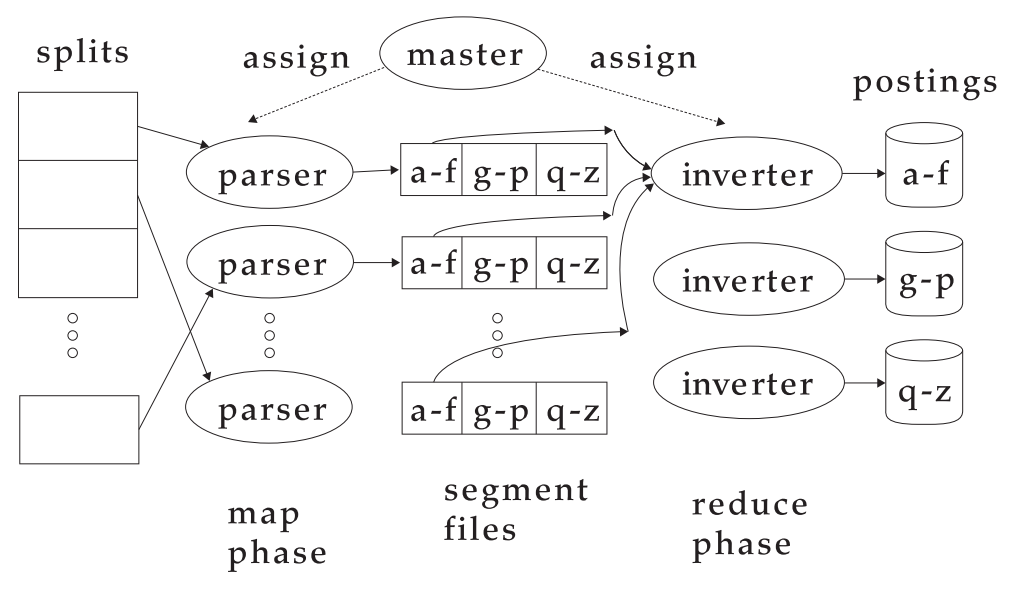
\includegraphics[scale=0.40]{sect4/figure_4_5.png}
    \caption{An example of distributed indexing with MapReduce.}
\end{figure}

Collecting all values for a given key into one list is the task of the \textbf{inverters}. The master assigns each term partition to a different inverter. Finally, the list of values is sorted for each key and written to the final sorted postings list.

Parsers and inverters are not separate sets of machines. The master identifies idle machines and assigns tasks to them. The same machine can be a parser in the map phase and an inverter in the reduce phase.

To minimize write times before inverters reduce the data, each parser writes its segment files to its \textbf{local disk}. In the reduce phase, the master communicates to an inverter the locations of the relevant segment files. Each segment file only requires one sequential read. This setup minimizes the amount of network traffic needed during indexing. Input and output are often lists of key-value pairs themselves, so that several MapReduce jobs can run in sequence.

\begin{figure}[H]
    \centering
    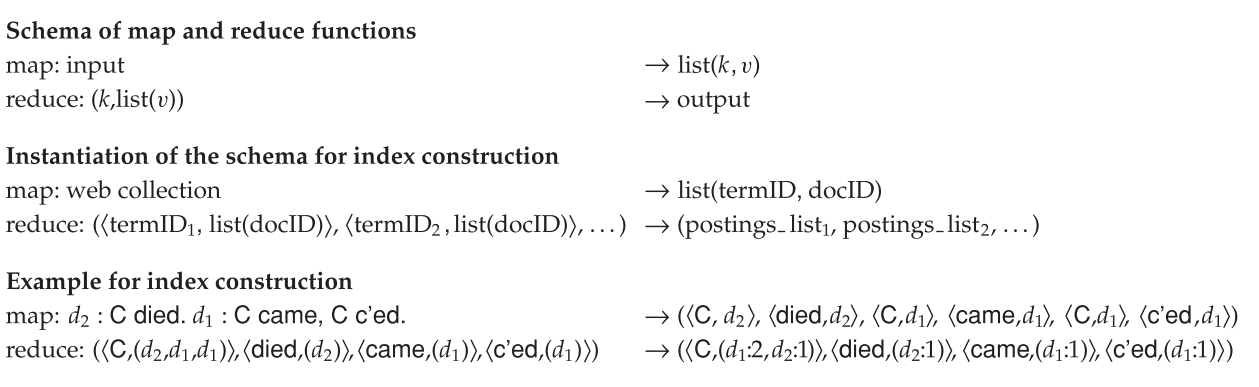
\includegraphics[scale=0.45]{sect4/figure_4_6.png}
    \caption{Map and reduce functions in MapReduce.}
\end{figure}

\subsection{Dynamic indexing}
Most collections are modified frequently with documents being added, deleted, and updated. New terms need to be added to the dictionary, and postings lists need to be updated.

The simplest way to achieve this is to periodically reconstruct the index from scratch. This is a good solution if the number of changes over time is small and if enough resources are available to construct a new index while the old one is still available for querying.

If there is a requirement that new documents be included quickly, one solution is to maintain two indexes: a large main index and a small \textbf{auxiliary index} that stores new documents. The auxiliary index is kept in memory. Searches are run across both indexes. Deletions are stored in an invalidation bit vector. We can then filter out deleted documents before returning the search result.

Each time the auxiliary index becomes too large, we merge it into the main index. The cost of this merging operation depends on how we store the index. If we store each postings list as a separate file, then the merge consists of extending each postings list of the main index by the corresponding postings list of the auxiliary index.

Unfortunately, the one-file-per-postings-list scheme is infeasible because most file systems cannot efficiently handle very large numbers of files. The simplest alternative is to store the index as one large file as a concatenation of all postings lists. In reality, we often choose a compromise between the two extremes.

In a scheme where the index is one big file, we process each posting $\left \lfloor{T/n}\right \rfloor$ times because we touch it during each of $\left \lfloor{T/n}\right \rfloor$ merges where n is the size of the auxiliary index and $T$ the total number of postings. Thus, the time complexity is $\Theta(T^2/n)$. We can do better with a scheme called \textbf{logarithmic merging}. Logarithmic merging amortizes the cost of merging indexes over time. As before, up to $n$ postings are accumulated in an in-memory auxiliary index, which we call $Z_0$. When the limit $n$ is reached, the $2^0 \times n$ postings in $Z_0$ are transferred to a new index $I_0$ that is created on disk. The next time $Z_0$ is full, it is merged with $I_0$ to create an index $Z_1$ of size $2^1 \times n$. Then $Z_1$ is either stored as $I_1$ (if there isn’t already an $I_1$) or merged with $I_1$ into $Z_2$ (if $I_1$ exists); and so on.

Overall index construction time is $\Theta(T \log(T/n))$ because each posting is processed only once on each of the $\log(T/n)$ levels. We trade this efficiency gain for a slow down of query processing; we now need to merge results from $\log(T/n)$. We still need to merge very large indexes occasionally, but this happens less frequently.

Because of this complexity of dynamic indexing, some large search engines adopt a reconstruction-from-scratch strategy. They do not construct indexes dynamically. Instead, a new index is built from scratch periodically. Query processing is then switched from the new index and the old index is deleted.

\section{Index compression}
Compression techniques for dictionary and inverted index are essential for efficient IR systems. One benefit of compression is straightforward: we need less disk space. 

There are two more benefits of compression. The first is increased use of caching. Search systems use some parts of the dictionary much more than others. If we cache the postings list of a frequently used query term $t$, then the computations necessary for responding to t can be entirely done in memory. With compression, we can fit a lot more information into main memory.

The second advantage of compression is faster transfer of data from disk to memory. Efficient decompression algorithms run so fast on modern hardware that the total time of transferring a compressed chunk of data from disk and then decompressing it is usually less than transferring the same chunk of data in uncompressed form. In most cases, the retrieval system runs faster on compressed postings lists than on uncompressed postings lists.

We define a \textbf{posting} as a docID in a postings list. For example, the postings list (6; 20, 45, 100), where 6 is the termID, contains three postings.

\subsection{Statistical properties of terms in information retrieval}

Reuters-RCV1 will be our model collection. \ref{RCV1-table} shows the preprocessing affects the size of the dictionary and the number of nonpositional postings. Stemming and case folding reduce the number of (distinct) terms by $17\%$ each and the number of nonpositional postings by 4\% and 3\%, respectively. Eliminating the 150 most common words from indexing cuts 25\% to 30\% of the nonpositional postings. But this size reduction does not carry over to the size of the compressed index. The postings lists of frequent words require only a few bits per posting after compression. However, the the percentage reductions can be very different for some text collections. For example, for a collection of web pages with a high proportion of French text, a lemmatizer for French reduces vocabulary size much more than the Porter stemmer does for an English-only collection because French is a morphologically richer language than English.

\begin{figure}[H]
    \centering
    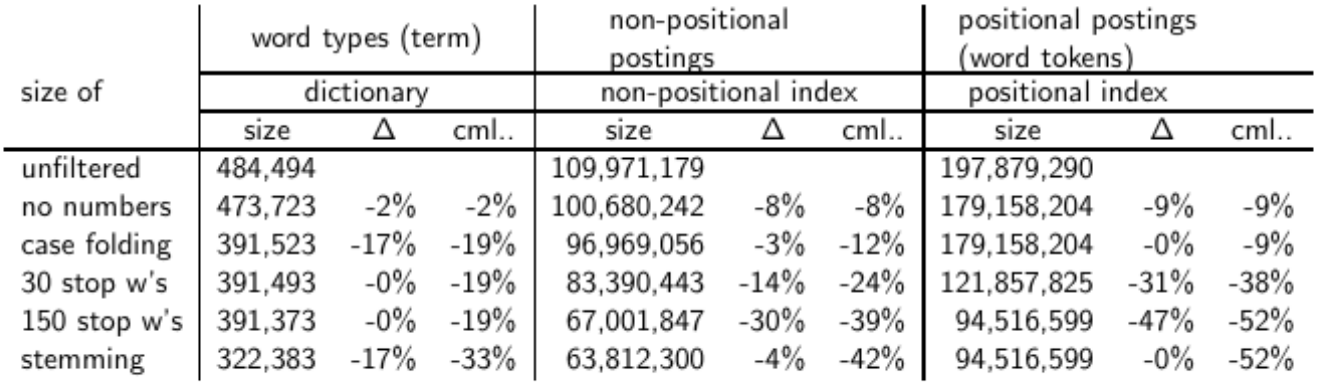
\includegraphics[scale=0.40]{sect5/table_5_1.png}
    \caption{The effect of preprocessing on the number of terms, nonpositional postings, and tokens for Reuters-RCV1.}
    \label{RCV1-table}
\end{figure}

The compression techniques are \textbf{lossless}, where all information is preserved, and \textbf{lossy}, which discards some information. Case folding, stemming, and stop word elimination are forms of lossy compression. The vector space model and dimensionality reduction techniques like latent semantic indexing create compact representations from which we cannot fully restore the original collection. Lossy compression makes sense when the “lost” information is unlikely ever to be used.

Before introducing techniques for compressing the dictionary, it's useful to estimate the number of distinct terms $M$ in a collection. The second edition of the \textit{Oxford English Dictionary} (OED) defines more than 600,000 words, but it does not include most names of people, locations, products, etc. These names need to be included in the inverted index.

\subsection{Heaps’ law: Estimating the number of terms}
A better way of getting a handle on $M$ is \textbf{Heaps’ law}, which estimates vocabulary size as a function of collection size:
\[
M=kT^b
\]
where $T$ is the number of tokens in the collection. Typical values for the parameters $k$ and $b$ are: $30 \leq k \leq 100$ and $b \approx 0.5$.

Heaps’ law suggests that (i) the dictionary size continues to increase with more documents in the collection and (ii) the size of the dictionary is quite large for large collections.

\begin{figure}[H]
    \centering
    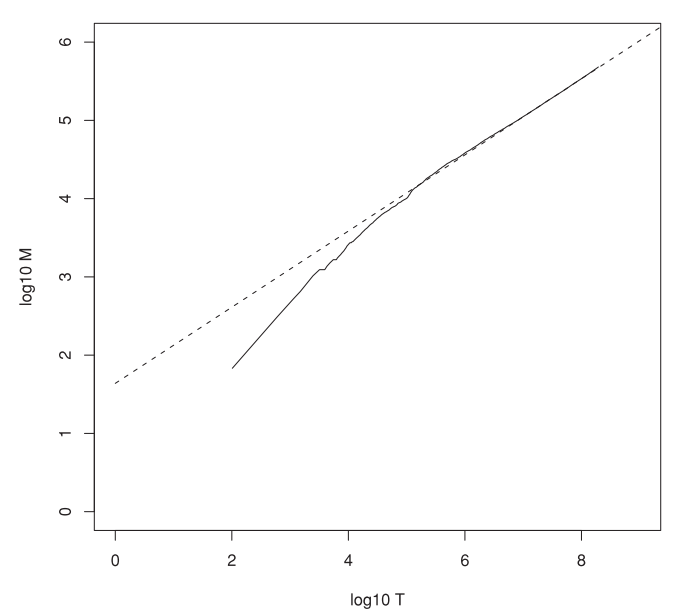
\includegraphics[scale=0.60]{sect5/figure_5_1.png}
    \caption{Heaps’ law. Vocabulary size $M$ as a function of collection size $T$ (number of tokens) for Reuters-RCV1.}
\end{figure}

\subsection{Zipf’s law: Modeling the distribution of terms}
We also want to understand how terms are distributed across documents. A commonly used model of the distribution of terms in a collection is \textbf{Zipf’s law}. It states that, if $t_1$ is the most common term in the collection, $t_2$ is the next most common, and so on, then the collection frequency $cf_i$ of the $i$th most common term is proportional to $1/i$:
\[
cf_i \propto \frac{1}{i}.
\]
So if the most frequent term occurs $cf_i$ times, then the second most frequent term has half as many occurrences, the third most frequent term a third as many occurrences, and so on. The frequency decreases very rapidly with rank.

Equivalently, we can write Zipf’s law as $cf_i=ci^k$ or as $\log cf_i=\log c + k\log i$ where $k=−1$ and $c$ is a constant. It is therefore a power law with exponent $k=−1$.

The fit of the data to the law is not particularly good, but good enough to serve as a model for term distributions.

\begin{figure}[H]
    \centering
    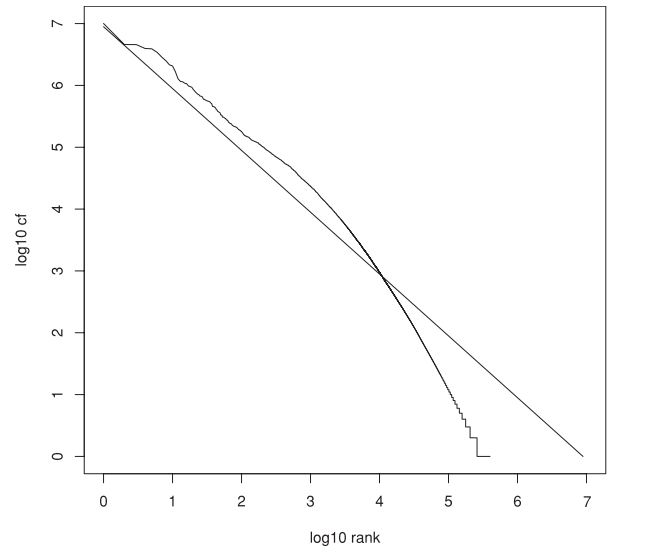
\includegraphics[scale=0.60]{sect5/figure_5_2.png}
    \caption{Zipf’s law for Reuters-RCV1. Frequency is plotted as a function of frequency rank for the terms in the collection. The line is the distribution predicted by Zipf’s law.}
\end{figure}

\subsection{Dictionary compression}
One of the primary factors in determining the response time of an IR system is the number of disk seeks necessary to process a query. If parts of the dictionary are on disk, then many more disk seeks are necessary in query evaluation. Thus, the main goal of compressing the dictionary is to fit it in main memory, 

\paragraph{Dictionary as a string}
The simplest data structure for the dictionary is to sort the vocabulary lexicographically and store it in an array of fixed-width entries. We allocate 20 bytes for the term itself, 4 bytes for its document frequency, and 4 bytes for the pointer to its postings list. Four-byte pointers resolve a 4 GB address space. For large collections like the web, we need to allocate more bytes per pointer. We look up terms in the array by binary search. For Reuters-RCV1, we need $M \times (20 + 4 + 4) = 400,000\times28 = 11.2$ MB for storing the dictionary in this scheme.
\begin{figure}[H]
    \centering
    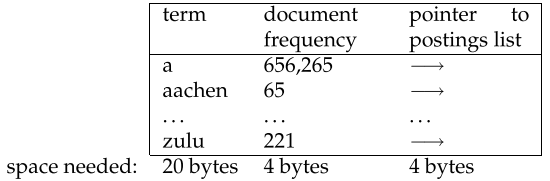
\includegraphics[scale=0.60]{sect5/figure_5_3.png}
    \caption{Storing the dictionary as an array of fixed-width entries.}
\end{figure}

Using fixed-width entries for terms is wasteful. The average length of a term in English is about eight characters. Also, we have no way of storing terms with more than twenty characters like \code{hydrochlorofluorocarbons} and \code{supercalifragilisticexpialidocious}. We can overcome these shortcomings by storing the dictionary terms as one long string of characters. The pointer to the next term is also used to demarcate the end of the current term. This scheme saves us 60\% compared to fixed-width storage (12 bytes on average of the 20 bytes). However, we now also need to store term pointers. The term pointers resolve $400,000 \times 8 = 3.2\times10^6$ positions, so they need to be $\log_2 3.2 × 10^6\approx22$ bits or 3 bytes long.

In this new scheme, we need $400,000 \times (4 + 4 + 3 + 8) = 7.6$ MB for the Reuters-RCV1 dictionary: 4 bytes each for frequency and postings pointer, 3 bytes for the term pointer, and 8 bytes on average for the term. So we have reduced the space from 11.2 to 7.6 MB.
\begin{figure}[H]
    \centering
    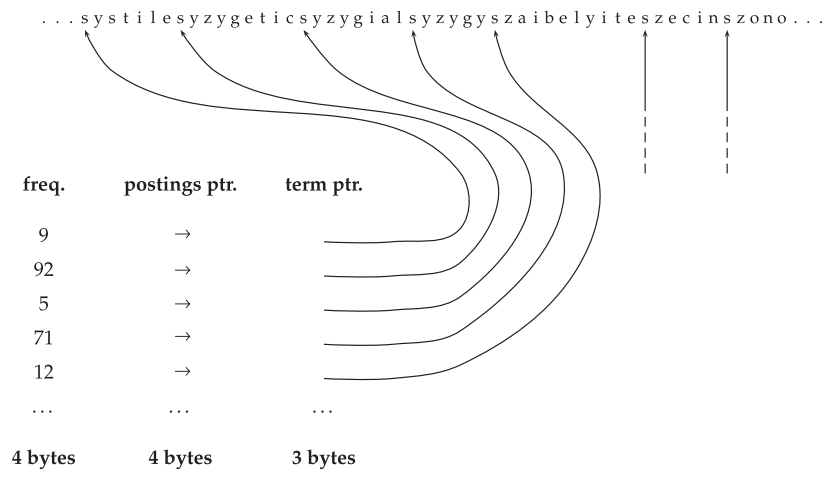
\includegraphics[scale=0.60]{sect5/figure_5_4.png}
    \caption{Dictionary-as-a-string storage. Pointers mark the end of the preceding term and the beginning of the next. For example, the first three terms in this example are \code{systile}, \code{syzygetic}, and \code{syzygial}.}
\end{figure}

\paragraph{Blocked storage}
We can further compress the dictionary by grouping terms in the string into blocks of size $k$ and keeping a term pointer only for the first term of each block. We store the length of the term in the string as an additional byte at the beginning of the term. We thus eliminate $k − 1$ term pointers, but need an additional $k$ bytes for storing the length of each term. For $k = 4$, we save $(k − 1) \times 3 = 9$ bytes for term pointers, but need an additional $k = 4$ bytes for term lengths. So the total space requirements for the dictionary of Reuters-RCV1 are reduced by 0.5 MB, to 7.1 MB.
\begin{figure}[H]
    \centering
    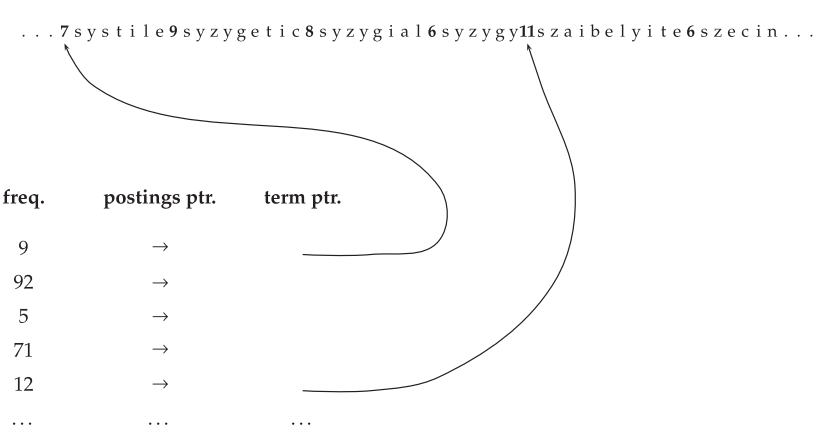
\includegraphics[scale=0.55]{sect5/figure_5_5.png}
    \caption{Blocked storage with four terms per block. The first block consists of \code{systile}, \code{syzygetic}, \code{syzygial}, and \code{syzygy} with lengths of seven, nine, eight, and six characters, respectively. Each term is preceded by a byte encoding its length that indicates how many bytes to skip to reach subsequent terms.}
\end{figure}

By increasing the block size k, we get better compression. However, there is a tradeoff between compression and the speed of term lookup. We search for terms in the uncompressed dictionary by binary search (a). In the compressed dictionary, we first locate the term’s block by binary search and then its position within the list by linear search through the block (b). Searching the uncompressed dictionary in (a) takes on average $(0 + 1 + 2 + 3 + 2 + 1 + 2 + 2)/8\approx1.6$ steps. With blocks of size k = 4 in (b), we need $(0+1+2+3+4+1+2+3)/8 = 2$ steps on average, $\approx25\%$ more.
\begin{figure}[H]
    \centering
    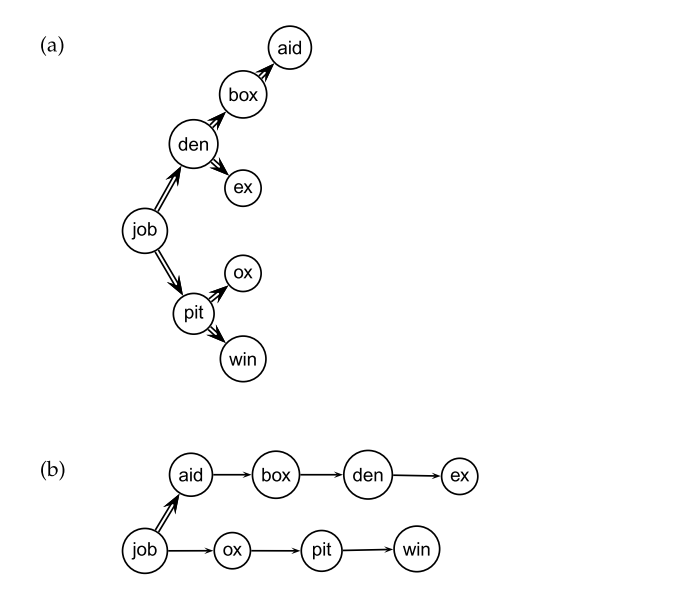
\includegraphics[scale=0.55]{sect5/figure_5_6.png}
    \caption{Search of the uncompressed dictionary (a) and a dictionary compressed by blocking with $k = 4$ (b).}
\end{figure}

Consecutive entries in an alphabetically sorted list share common prefixes. This observation leads to \textbf{front coding}. A common prefix is identified for a subsequence of the term list and then referred to with a special character. In the case of Reuters, front coding saves another 1.2 MB.
\begin{figure}[H]
    \centering
    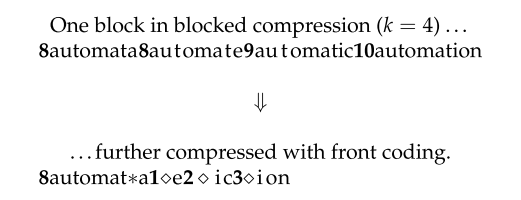
\includegraphics[scale=0.60]{sect5/figure_5_7.png}
    \caption{Front coding. A sequence of terms with identical prefix (“automat”) is encoded by marking the end of the prefix with $∗$ and replacing it with ⋄ in subsequent terms. As before, the first byte of each entry encodes the number of characters.}
\end{figure}
\begin{figure}[H]
    \centering
    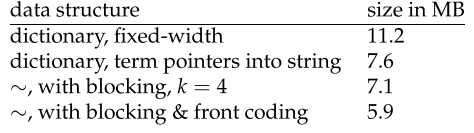
\includegraphics[scale=0.60]{sect5/table_5_2.png}
    \caption{Dictionary compression for Reuters-RCV1.}
\end{figure}

\subsection{Postings file compression}
Reuters-RCV1 has 800,000 documents, 200 tokens per document, six characters per token, and 100,000,000 postings. Document identifiers are $\log_2 800,000\approx20$ bits long. Thus, the size of the collection is about $800,000\times200\times6$ bytes $= 960$ MB and the size of the uncompressed postings file is $100,000,000\times20/8 = 250$ MB.

To devise a more efficient representation of the postings file, one that uses fewer than 20 bits per document, we observe that the postings for frequent terms are close together. The key idea is that the \textbf{gaps} between postings are short. In fact, gaps for the most frequent terms are mostly equal to 1. But the gaps for a rare term need 20 bits. For an economical representation of this distribution of gaps, we need a variable encoding method that uses fewer bits for short gaps. To encode small numbers in less space than large numbers, we look at two types of methods: bytewise compression and bitwise compression.

\paragraph{Variable byte codes}
\textbf{Variable byte} (\textbf{VB}) \textbf{encoding} uses an integral number of bytes to encode a gap. The last 7 bits of a byte are “payload” and encode part of the gap. The first bit of the byte is a \textbf{continuation bit}. It is set to 1 for the last byte of the encoded gap and to 0 otherwise. To decode a variable byte code, we read a sequence of bytes with continuation bit 0 terminated by a byte with continuation bit 1. We then extract and concatenate the 7-bit parts.
\begin{figure}[H]
    \centering
    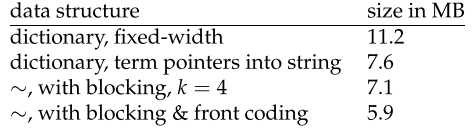
\includegraphics[scale=0.60]{sect5/table_5_4.png}
    \caption{VB encoding. Gaps are encoded using an integral number of bytes. The first bit, the continuation bit, of each byte indicates whether the code ends with this byte (1) or not (0).}
\end{figure}
With VB compression, the size of the compressed index for Reuters-RCV1 is 116 MB. This is a more than 50\% reduction of the size of the uncompressed index. 

The idea of VB encoding can also be applied to larger or smaller units than bytes: 32-bit words, 16-bit words, and 4-bit words or \textit{nibbles}. Bytes offer a good compromise between compression ratio and speed of decompression. They are also simple to implement. 

We can achieve better compression ratios by using bit-level encodings, in particular two closely related encodings: $\gamma$ codes, which we will turn to next, and $\delta$ codes.

\paragraph{$\gamma$ codes}
VB codes use an adaptive number of bytes depending on the size of the gap. Bit-level codes adapt the length of the code on the finer grained bit level. The simplest bit-level code is \textbf{unary code}. The unary code of $n$ is a string of $n$ 1s followed by a 0. This is not a very efficient code.

Assuming the $2^n$ gaps $G$ with $1 \leq G \leq 2^n$ are all equally likely, the optimal encoding uses $n$ bits for each $G$. So some gaps cannot be encoded with fewer than $\log_2 G$ bits. Our goal is to get as close to this lower bound as possible.

$\gamma$ codes implement variable-length encoding by splitting the representation of a gap $G$ into a pair of length and offset. \textbf{Offset} is $G$ in binary, but with the leading 1 removed. For example, for 13 (binary 1101) offset is 101. \textbf{Length} encodes the length of offset in unary code. For 13, the length of offset is 3 bits, which is 1110 in unary. The $\gamma$ code of 13 is therefore 1110101.
\begin{figure}[H]
    \centering
    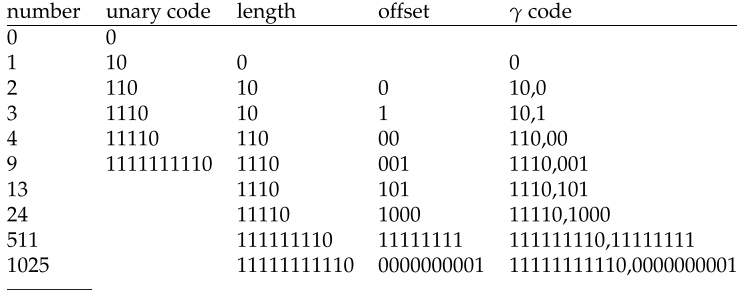
\includegraphics[scale=0.60]{sect5/table_5_5.png}
    \caption{Some examples of unary and $\gamma$ codes. Unary codes are only shown for the smaller numbers. Commas in $\gamma$ codes are for readability only and are not part of the actual codes.}
\end{figure}

A $\gamma$ code is decoded by first reading the unary code up to the 0 that terminates it, for example, the four bits 1110 when decoding 1110101. Now we know how long the offset is: 3 bits. The offset 101 can then be read correctly and the 1 that was chopped off in encoding is prepended: $101 \rightarrow 1101 = 13$. The length of offset is $\left \lfloor{\log_2 G}\right \rfloor$ bits and the length of length is $\left \lfloor{\log_2 G + 1}\right \rfloor$ bits, so the length of the entire code is $2 \times \left \lfloor{\log_2 G + 1}\right \rfloor$1 bits. $\gamma$ codes are always of odd length and they are within a factor of 2 of what we claimed to be the optimal encoding length $\log_2 G$.

$\gamma$ codes have two other properties. First, they are \textbf{prefix free}, no $\gamma$ code is the prefix of another. This means that there is always a unique decoding of a sequence of $\gamma$ codes – and we do not need delimiters between them. The second property is that $\gamma$ codes are parameter free.

\begin{figure}[H]
    \centering
    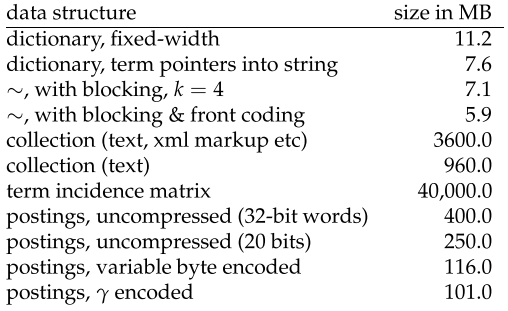
\includegraphics[scale=0.60]{sect5/table_5_6.png}
    \caption{Index and dictionary compression for Reuters-RCV1. The compression ratio depends on the proportion of actual text in the collection. Reuters-RCV1 contains a large amount of XML markup. Using the two best compression schemes, $\gamma$ encoding and blocking with front coding, the ratio compressed index to collection size is therefore especially small for Reuters-RCV1: $(101 + 5.9)/3600\approx0.03$.}
\end{figure}

\section{Scoring, term weighting and the vector space model}
In the case of large document collections, the resulting number of matching documents can far exceed the number a human user could possibly sift through. It is essential for a search engine to rank-order the documents matching a query. To do this, the search engine computes a score with respect to the query.

\subsection{Parametric and zone indexes}
Digital documents generally encode certain \textbf{metadata} associated with each document. This metadata would generally include fields such as the date of creation and the format of the document.

Consider queries of the form “find documents authored by William Shakespeare in 1601, containing the phrase \code{alas poor Yorick}”. Query processing then consists as usual of postings intersections from standard inverted as well as\textbf{ parametric indexes}. There is one parametric index for each field; it allows us to select only the documents matching a date specified in the query.

\textbf{Zones} are similar to fields, except the contents of a zone can be arbitrary
free text. A zone can be thought of as an arbitrary, unbounded amount of text. For instance, document titles and abstracts are generally treated as zones. We may build a separate inverted index for each zone of a document, to support queries such as “find documents with \code{merchant} in the title and \code{william} in the author list and the phrase \code{ gentle rain} in the body”. Whereas the dictionary for a parametric index comes from a fixed vocabulary, the dictionary for a zone index must structure whatever vocabulary stems from the text of that zone.

We can reduce the size of the dictionary by encoding the zone in which a term occurs in the postings, a technique called \textbf{weighted zone scoring}.
\begin{figure}[H]
    \centering
    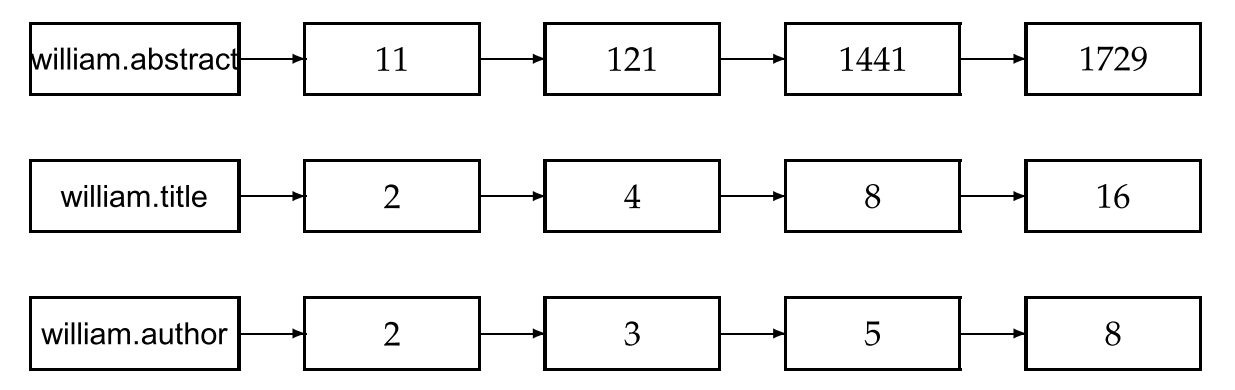
\includegraphics[scale=0.50]{sect6/figure_6_2.png}
    \caption{Basic zone index ; zones are encoded as extensions of dictionary entries.}
\end{figure}
\begin{figure}[H]
    \centering
    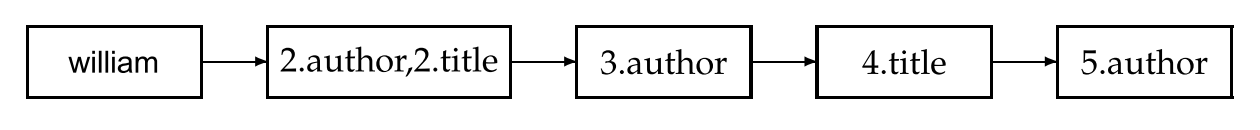
\includegraphics[scale=0.50]{sect6/figure_6_3.png}
    \caption{Zone index in which the zone is encoded in the postings rather than the dictionary.}
\end{figure}

\paragraph{Weighted zone scoring}
Given a Boolean query $q$ and $a$ document $d$, weighted zone scoring assigns to the pair $(q, d)$ a score in the interval $[0, 1]$, by computing a linear combination of \textbf{zone scores}. Consider a set of documents each of which has $\ell$ zones. Let $g_1,\dots,g_\ell \in [0,1]$ such that $\sum_{i=1}^{\ell}g_i=1$. For $1\leq i \leq \ell$, let $s_i$ be the Boolean score denoting a match between $q$ and the $i$th zone. The weighted zone score is defined to be
\[
\sum_{i=1}^{\ell}g_is_i
\]
Weighted zone scoring is sometimes referred to also as \textbf{ranked Boolean retrieval}.

A simple approach to implement the computation of weighted zone scores would be to compute scores directly from inverted indexes. The algorithm scan the postings traversal adding a document to the set of results for a Boolean AND query and computing a score for each such document.

\paragraph{Learning weights}
The weights $g_i$ for weighted zone scoring could be specified by an expert, or learned using training examples that have been judged editorially (\textbf{machine-learned relevance}). The basic steps of a machine-learned relevance approach are:
\begin{itemize}
    \item We are provided with a set of training examples, a set of tuple consisting of a query $q$ and a document $d$, with a relevance judgment for $d$ on $q$.
    \item The weights $g_i$ are then “learned” from these examples, in order that the learned scores approximate the relevance judgments in the training examples.
\end{itemize}
The process may be viewed as learning a linear function of the Boolean match scores contributed by the various zones.

\subsection{Term frequency and weighting}

A document or zone that mentions a query term more often has more to do with that query and therefore should receive a higher score.We assign to each term in a document a weight for that term, that depends on the number of occurrences of the term in the document. We would like to compute a score between a query term $t$ and a document $d$, based on the weight of $t$ in $d$. The simplest approach is to assign the weight to be equal to the number of occurrences of $t$ in $d$. This weighting scheme is referred to as \textbf{term frequency} and is denoted tf$_{t,d}$.

For a document $d$, the set of weights determined by the tf weights may be viewed as a quantitative digest of that document. In this view of a document, called \textbf{bag of words model}, the exact ordering of the terms in a document is ignored.

\paragraph{Inverse document frequency}
Raw term frequency as above suffers from a critical problem: all terms are considered equally important when it comes to assessing relevancy on a query. For instance, a collection of documents on the auto industry is likely to have the term auto in almost every document. Thus we introduce a mechanism for attenuating the effect of terms that occur too often.

The \textbf{document frequency} df$_t$, defined to be the number of documents in the collection that contain a term $t$. It is better to use a document-level statistic than to use a collection-wide statistic for the term. \ref{figure_25} shows that collection frequency (cf) and document frequency (df) can behave rather differently. In particular, the cf values for both \code{try} and \code{insurance} are roughly equal, but their df values differ significantly. We want the few documents that contain \code{insurance} to get a higher boost for a query on \code{insurance} than the many documents containing \code{try} get from a query on \code{try}.
\begin{figure}[H]
    \centering
    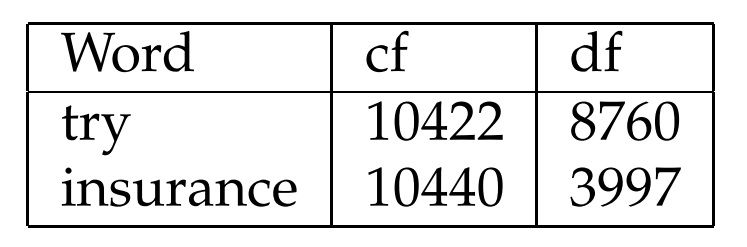
\includegraphics[scale=0.30]{sect6/figure_6_7.png}
    \caption{Collection frequency (cf) and document frequency (df) behave differently, as in this example from the Reuters collection.}
    \label{figure_25}
\end{figure}

How is the document frequency df of a term used to scale its weight? Denoting total number of documents in a collection by $N$, we define the \textbf{inverse document frequency} (idf) of a term $t$ as follows:
\[
\textrm{idf}_t=\log\frac{N}{\textrm{df}_t}
\]
Thus the idf of a rare term is high, whereas the idf of a frequent term is likely to be low.

\paragraph{Tf-idf weighting}
We now combine the definitions of term frequency and inverse document frequency, to produce a composite weight for each term in each document. The \textbf{tf-idf} weighting scheme assigns to term $t$ a weight in document $d$ given by
\[
\textrm{tf-idf}_{t,d}=\textrm{tf}_{t,d}\times \textrm{idf}_{t}
\]
tf-idf$_{t,d}$ assigns to term $t$ a weight in document $d$ that is
\begin{enumerate}
    \item highest when $t$ occurs many times within a small number of documents
    \item lower when the term occurs fewer times in a document, or occurs in many documents
    \item lowest when the term occurs in virtually all documents.
\end{enumerate}

We may view each document as a \textbf{vector} with one component
corresponding to each term in the dictionary, together with a weight for each component. For dictionary terms that do not occur in a document, this weight is zero.

Now we introduce the \textbf{overlap score measure}: the score of a document $d$ is the sum, over all query terms, of the number of times each of the query terms occurs in $d$. We add up not the number of occurrences of each query term $t$ in $d$, but instead the tf-idf weight of each term in $d$.
\[
\textrm{Score}(q,d)=\sum_{t \in q}\textrm{tf-idf}_{t,d}.
\]

\subsection{The vector space model for scoring}
The representation of a set of documents as vectors in a common vector space is known as the \textbf{vector space model}.

\paragraph{Dot products}
We denote by $\vec{V}(d)$ the vector derived from document $d$, with one component in the vector for each dictionary term. The set of documents in a collection then may be viewed as a set of vectors in a vector space, in which there is one axis for each term. This representation loses the relative ordering of the terms in each document.

How do we quantify the similarity between two documents in this vector
space? A first attempt might consider the magnitude of the vector difference between two document vectors, but this measure suffers from a drawback: two documents with very similar content can have a significant vector difference simply because one is much longer than the other.

To compensate for the effect of document length, the standard way of quantifying the similarity between two documents $d_1$ and $d_2$ is to compute the cosine similarity of their vector representations $\vec{V}(d_1)$ and $\vec{V}(d_2)$
\[
\textrm{sim}(d_1,d_2)=\frac{\vec{V}(d_1) \cdot \vec{V}(d_2)}{|\vec{V}(d_1)||\vec{V}(d_2)|}
\]
where the numerator represents the dot product of the vectors $\vec{V}(d_1)$ and $\vec{V}(d_2)$, while the denominator is the product of their\textbf{ Euclidean lengths}. The effect of the denominator is to length-normalize the vectors $\vec{V}(d_1)$ and $\vec{V}(d_2)$ to unit vectors $\vec{v}(d_1) = \vec{V}(d_1)/|\vec{V}(d_1)|$ and $\vec{v}(d_2) = \vec{V}(d_2)/|\vec{V}(d_2)|$. We can then rewrite the equation as
\[
\textrm{sim}(d_1,d_2)=\vec{v}(d_1) \cdot \vec{v}(d_2).
\]
It can be viewed as the dot product of the normalized versions of the two document vectors. This measure is the cosine of the angle $\Theta$ between the two vectors. Given a document $d$, consider searching for the documents in the collection most similar to $d$. Such a search is useful in a system where a user may identify a document and seek others like it. We reduce the problem of finding the document(s) most similar to $d$ to that of finding the $d_i$ with the highest dot products $\vec{v}(d) \cdot \vec{v}(d_i)$.

Viewing a collection of $N$ documents as a collection of vectors leads to a natural view of a collection as a term-document matrix: this is an $M \times N$ matrix whose rows represent the $M$ terms (dimensions) of the $N$ columns, each of which corresponds to a document.
\begin{figure}[H]
    \centering
    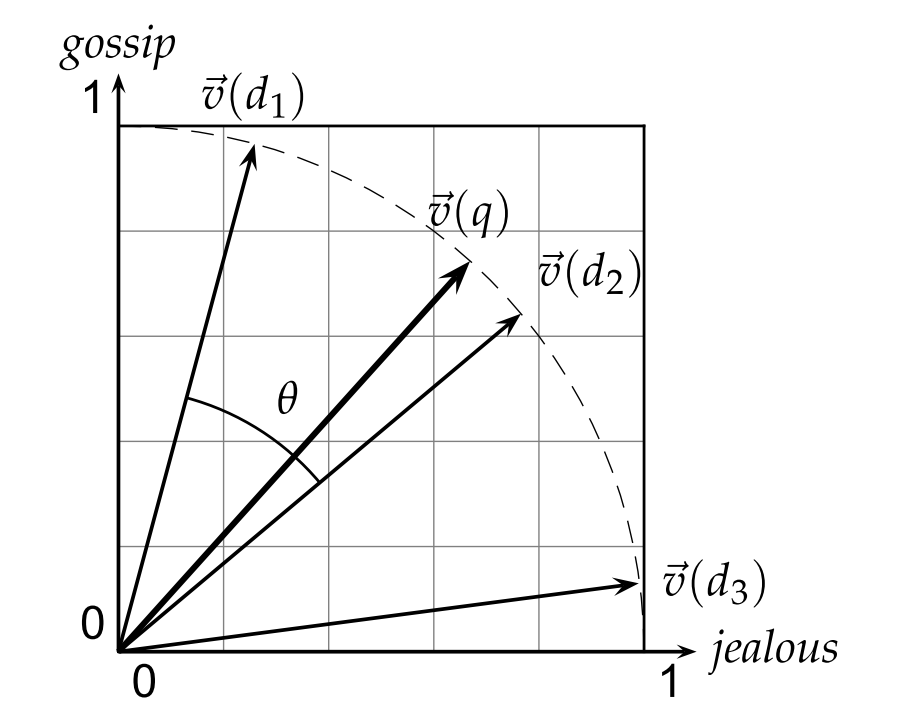
\includegraphics[scale=0.40]{sect6/figure_6_10.png}
    \caption{Cosine similarity illustrated. $\textrm{sim}(d_1,d_2)=\cos{\Theta}$.}
\end{figure}

\paragraph{Queries as vectors}
We can also view a query as a vector. Consider a query $q$. This query turns into the unit vector $\vec{v}(q)$. The idea is to assign to each document $d$ a score equal to the dot product
\[
\vec{v}(q) \cdot \vec{v}(d).
\]

By viewing a query as a “bag of words”, we are able to treat it as a very short document. We can use the cosine similarity between the query vector and a document vector as a measure of the score of the document for that query. The resulting scores can then be used to select the top-scoring documents for a query. Thus we have
\[
\textrm{Score}(q,d)=\frac{\vec{V}(q) \cdot \vec{V}(d)}{|\vec{V}(q)||\vec{V}(d)|}
\]
A document may have a high cosine score for a query even if it does not contain all query terms.

Computing the cosine similarities between the query vector and each document vector in the collection, sorting the resulting scores and selecting the top $K$ documents can be expensive.

\paragraph{Computing vector scores}
In a typical setting we have a collection of documents each represented by a vector, a free text query represented by a vector, and a positive integer $K$. We seek the $K$ documents of the collection with the highest vector space scores on the given query. Typically, we seek these $K$ top documents in ordered by decreasing score (for instance many search engines use $K = 10$).

The Algorithm 4 computes the vector space scores. The array Length holds the lengths for each of the $N$ documents, whereas the array Scores holds the scores for each of the documents. When the scores are finally computed, all that remains is to pick off the $K$ documents with the highest scores. The outermost loop repeats the updating of Scores, iterating over each query term $t$ in turn. We calculate the weight in the query vector for term $t$. We update the score of each document by adding in the contribution from term $t$. This process is known as \textbf{term-at-a-time} scoring or accumulation, and the $N$ elements of the array Scores are therefore known as \textbf{accumulators}. It is wasteful to store the weight wf$_{t,d}$ of term $t$ in document $d$ since storing this weight may require a floating point number. Two ideas help. First, if we are using inverse document frequency, we need not precompute idf$_t$; it suffices to store $N/\textrm{df}_t$ at the head of the postings for $t$. Second, we store the term frequency tf$_{t,d}$ for each postings entry. Finally extracts the top $K$ scores: this requires a priority queue data structure, often implemented using a heap. Each of the $K$ top scores can be extracted from the heap at a cost of $O(\log N)$ comparisons.
\begin{algorithm}[H] 
\begin{algorithmic}[1]
\label{COSINE_SCORE} % and a label for \ref{} commands later in the document
\caption{The basic algorithm for computing vector space scores.}
\Function{COSINE\_SCORE}{$q$}
    \State $\textrm{float } Scores[N] = 0$
    \State $\textrm{Initialize } Length[N]$
    
    \ForAll{query term $t$}
        calculate $w_{t,q}$ and fetch postings list for $t$
        \ForAll{pair$(d, \textrm{tf}_{t,d})$ in postings list}
            Scores$[d] += wf_{t,d} \times w_{t,q}$
        \EndFor
    \EndFor
    \State $\textrm{Read the array } Length[d]$
    \ForAll{$d$}
        $Scores[d] = Scores[d]/Length[d]$
    \EndFor
    \State \Return $\textrm{Top } K \textrm{ components of } Scores[]$
\EndFunction
\end{algorithmic}
\end{algorithm}

\subsection{Variant tf-idf functions}
For assigning a weight for each term in each document, a number of alternatives to tf and tf-idf have been considered.

\paragraph{Sublinear tf scaling}
It seems unlikely that twenty occurrences of a term in a document truly carry twenty times the significance of a single occurrence. We can use instead the logarithm of the term frequency, which assigns a weight given by
\[
\textrm{wf}_{t,d} = \begin{cases} 1+\log\textrm{tf}_{t,d} & \textrm{if } \textrm{tf}_{t,d} > 0 \\ 0 & \textrm{otherwise} \end{cases}
\]

In this form, we may replace tf by wf, to obtain:
\[
\textrm{wf-idf}_{t,d}=\textrm{wf}_{t,d} \times \textrm{idf}_t.
\]

\paragraph{Maximum tf normalization}
One well-studied technique is to normalize the tf weights of all terms occurring in a document by the maximum tf in that document. For each document $d$, let $\textrm{tf}_{max}(d) = \textrm{max}_{\tau \in d} \textrm{tf}_{\tau,d}$, where $\tau$ ranges over all terms in $d$. Then we compute a normalized term frequency for each term $t$ in document $d$ by
\[
\textrm{ntf}_{t,d} = a + (1 - a) \frac{\textrm{tf}_{t,d}}{\textrm{tf}_{\textrm{max}}(d)}\textrm{,} 
\]
where $a$ is the \textbf{smoothing term}, a value between 0 and 1, whose role is to damp the contribution of the second term, which may be viewed as a scaling down of tf by the largest tf value in $d$.

Maximum tf normalization does suffer from the following issues:
\begin{enumerate}
    \item The method is unstable in the following sense: a change in the stop word list can dramatically alter term weightings. It is hard to tune.
    \item A document may contain an outlier term with an unusually large number of occurrences of that term, not representative of the content of that document.
    \item a document in which the most frequent term appears roughly as often as many other terms should be treated differently from one with a more skewed distribution.
\end{enumerate}

\begin{figure}[H]
    \centering
    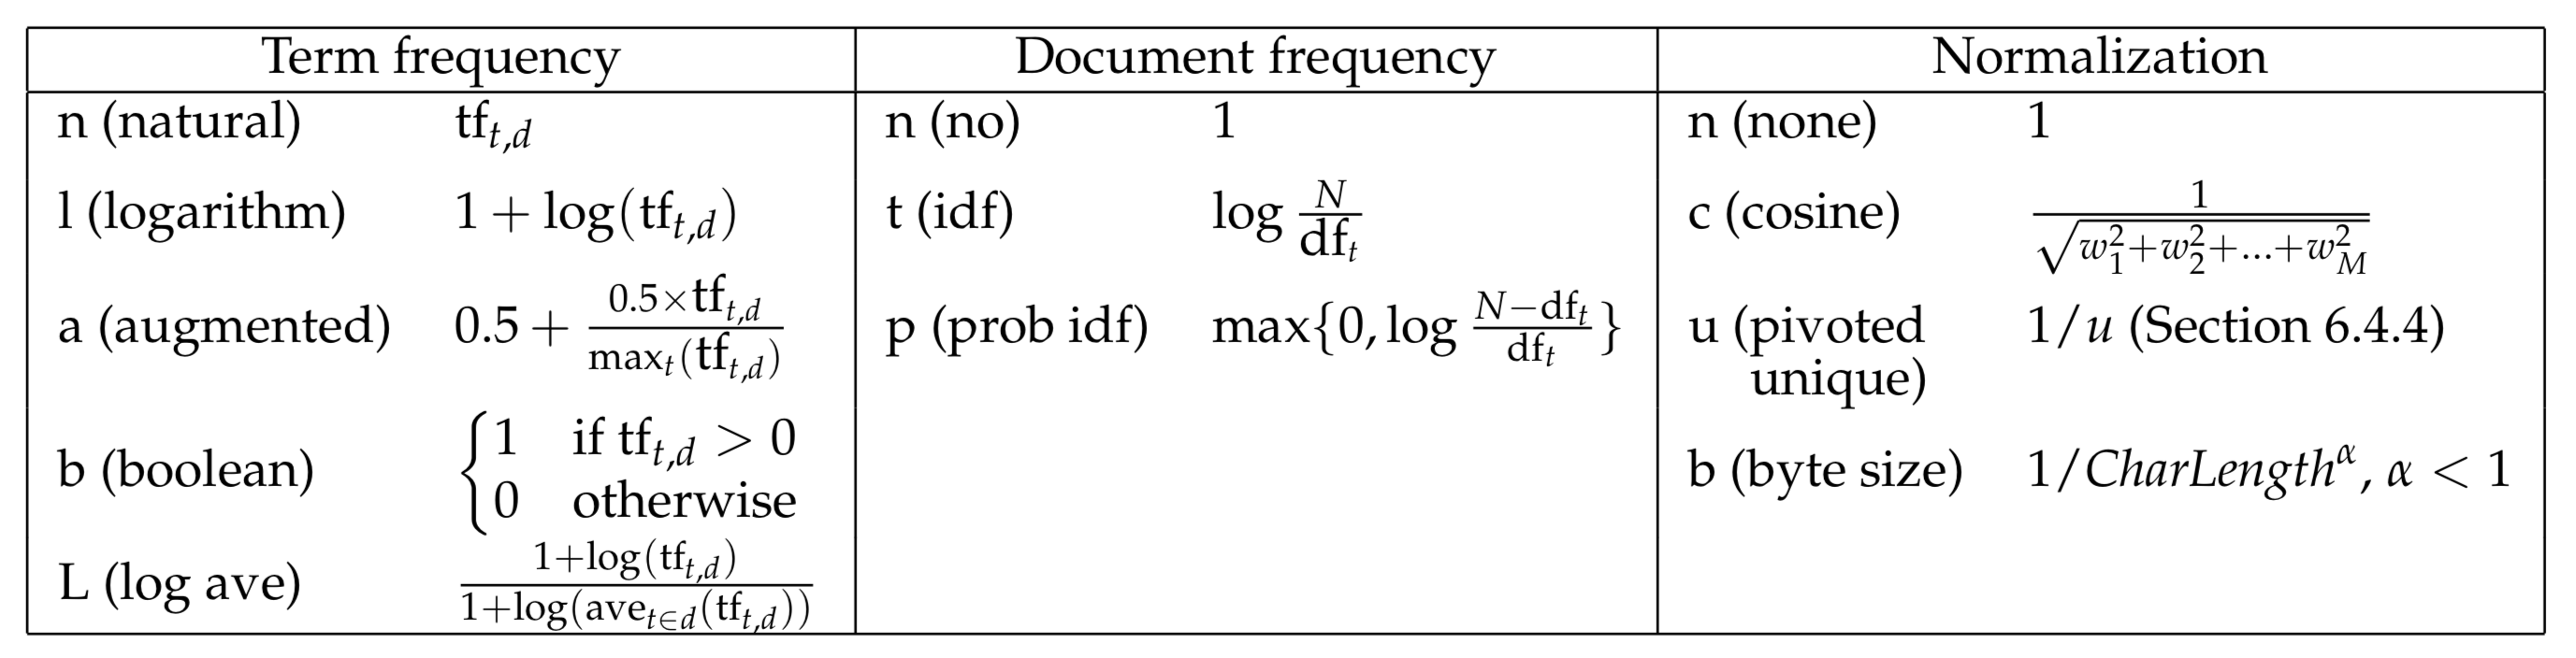
\includegraphics[scale=0.30]{sect6/figure_6_15.png}
    \caption{SMART notation for tf-idf variants. Here \textit{CharLength} is the number of characters in the document.}
\end{figure}

\section{Computing scores in a complete search system}

\subsection{Efficient scoring and ranking}
For a query such as $q =$ \code{jealous gossip}, two observations are immediate:
\begin{enumerate}
    \item The unit vector $\vec{v}(q)$ has only two non-zero components.
    \item In the absence of any weighting for query terms, these non-zero components are equal
\end{enumerate}

We are interested in the relative (rather than absolute) scores of the documents in the collection. To this end, it suffices to compute the cosine similarity from each document unit vector $\vec{v}(d)$ to $\vec{V}(q)$ (in which all non-zero components of the query vector are set to 1), rather than to the unit vector $\vec{v}(q)$. For any two documents $d_1$, $d_2$
\[
\vec{V}(q) \cdot \vec{v}(d_1) > \vec{V}(q) \cdot \vec{v}(d_2) \iff \vec{v}(q) \cdot \vec{v}(d_1) > \vec{v}(q) \cdot \vec{v}(d_2)
\]
For any document $d$, the cosine similarity $\vec{V}(q) \cdot \vec{v}(d)$ is the weighted sum, over all terms in the query $q$, of the weights of those terms in $d$. We walk through the postings in the inverted index for the terms in $q$, accumulating the total score for each document. We maintain an idf value for each dictionary term and a tf value for each postings entry. This scheme computes a score for every document in the postings of any of the query terms.

Given these scores, the final step before presenting results to a user is to pick out the $K$ highest-scoring documents. While one could sort the complete set of scores, a better approach is to use a heap to retrieve only the top $K$ documents in order. Where $J$ is the number of documents with non-zero cosine scores, constructing such a heap can be performed in $2J$ comparison steps, following which each of the $K$ highest scoring documents can be “read off” the heap with log $J$ comparison steps.

\paragraph{Inexact top K document retrieval}
Consider schemes by which we produce $K$ documents that are likely to be among the $K$ highest scoring documents for a query. We want to lower the cost of computing the $K$ documents we output, without materially altering the user’s perceived relevance of the top $K$ results. Consequently, in most applications it suffices to retrieve $K$ documents whose scores are very close to those of the $K$ best.

The \textbf{inexact top-$K$ retrieval} is not necessarily, from the user’s perspective, a bad thing. The top $K$ documents by the cosine measure are in any case not necessarily the $K$ best for the query: cosine similarity is only a proxy for the user’s perceived relevance. The heuristics have the following two-step scheme:
\begin{enumerate}
    \item Find a set $A$ of documents that are contenders, where $K < |A| < N$. $A$ does not necessarily contain the $K$ top-scoring documents for the query, but is likely to have many documents with scores near those of the top $K$.
    \item Return the $K$ top-scoring documents in $A$.
\end{enumerate}

\paragraph{Index elimination}
For a multi-term query $q$:
\begin{enumerate}
    \item We only consider documents containing terms whose idf exceeds a preset threshold. In the postings traversal, we only traverse the postings for terms with high idf. The postings lists of low-idf terms are generally long, thus the set of documents for which we compute cosines is greatly reduced. Low-idf terms are treated as stop words and do not contribute to scoring.
    \item We only consider documents that contain many of the query terms. A danger of this scheme is that by requiring all (or even many) query terms to be present in a document before considering it for cosine computation, we may end up with fewer than K candidate documents in the output.
\end{enumerate}

\paragraph{Champion lists}
The idea of \textbf{champion lists} is to precompute, for each term $t$ in the dictionary, the set of the $r$ documents with the highest weights for $t$. For tf-idf weighting, these would be the $r$ documents with the highest tf values for term $t$. We call this set of $r$ documents the champion list for term $t$.

Given a query $q$ we create a set $A$ as follows: we take the union of the champion lists for each of the terms comprising $q$. We restrict cosine computation to only the documents in $A$. A critical parameter is the value $r$. Intuitively, $r$ should be large compared with $K$. One issue here is that the value $r$ is set at the time of index construction, whereas $K$ is application dependent and may not be available until the query is received; as a result we may find ourselves with a set $A$ that has fewer than $K$ documents.

\paragraph{Static quality scores and ordering}
In many search engines, we have available a measure of quality $g(d) \in [0, 1]$ for each document $d$ that is query-independent and thus \textbf{static}.
\begin{figure}[H]
    \centering
    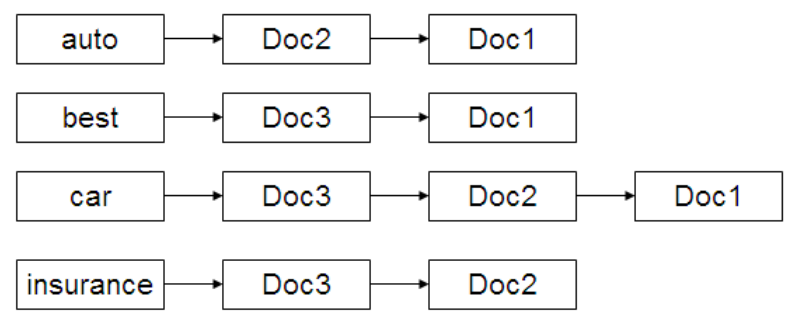
\includegraphics[scale=0.45]{sect7/figure_7_2.png}
    \caption{A static quality-ordered index. In this example we assume that Doc1, Doc2 and Doc3 respectively have static quality scores $g(1) = 0.25$, $g(2) = 0.5$, $g(3) = 1$.}
\end{figure}

The net score for a document $d$ is some combination of $g(d)$ together with the query-dependent score.
\[
\textrm{net-score}(q,d) = g(d) + \frac{\vec{V}(q) \cdot \vec{V}(d)}{|\vec{V}(q)| |\vec{V}(d)|}
\]
In this simple form, the static quality $g(d)$ and the query-dependent score have equal contributions. Other relative weightings are possible.

First, consider ordering the documents in the postings list for each term by decreasing value of $g(d)$. The first idea is a direct extension of champion lists: for a well-chosen value $r$, we maintain for each term $t$ a \textbf{global champion list} of the $r$ documents with the highest values for $g(d) + \textrm{tf-idf}_{t,d}$. The list itself is sorted by a common order. Then at query time, we only compute the net scores for documents in the union of these global champion lists.

We maintain for each term $t$ two postings lists consisting of disjoint sets of documents, each sorted by $g(d)$ values. The first list, which we call \textbf{high}, contains the $m$ documents with the highest tf values for $t$. The second list, which we call \textbf{low}, contains all other documents containing $t$. We first scan only the high lists of the query terms, if we obtain scores for $K$ documents in the process, we terminate. If not, we continue the scanning into the low lists.

\paragraph{Impact ordering}
In all the postings lists described thus far, we order the documents consistently by some common ordering. Such a common ordering supports the concurrent traversal of all of the query terms’ postings lists, computing the score for each document as we encounter it. Computing scores in this manner is sometimes referred to as document-at-a-time scoring. A inexact top-$K$ retrieval in which the postings are not all ordered by a common ordering requires scores to be “accumulated” one term at a time, so that we have term-at-a-time scoring.

The idea is to order the documents $d$ in the postings list of term $t$ by decreasing order of tf$_{t,d}$. Thus, the ordering of documents will vary from one postings list to another. Two ideas to significantly lower the number of documents for which we accumulate scores:
\begin{enumerate}
    \item When traversing the postings list for a query term $t$, we stop after considering a prefix of the postings list – either after a fixed number of documents $r$ have been seen, or after the value of tf$_{t,d}$ has dropped below a threshold
    \item When accumulating scores, we consider the query terms in decreasing order of idf, so that the query terms likely to contribute the most to the final scores are considered first.
\end{enumerate}

\paragraph{Cluster pruning}
In \textbf{cluster pruning} we have a preprocessing step during which we cluster the document vectors. Then at query time, we consider only documents in a small number of clusters as candidates for which we compute cosine scores. The preprocessing step is as follows:
\begin{enumerate}
    \item Pick $\sqrt{N}$ documents at random from the collection. Call these \textbf{leaders}.
    \item For each document that is not a leader, we compute its nearest leader.
\end{enumerate}
 We refer to documents that are not leaders as \textbf{followers}. The expected number of followers for each leader is $\approx N/\sqrt{N} = \sqrt{N}$. Next, the query processing proceeds as follows:
 \begin{enumerate}
    \item Given a query $q$, find the leader $L$ that is closest to $q$. This entails computing cosine similarities from $q$ to each of the $\sqrt{N}$ leaders.
    \item The candidate set $A$ consists of $L$ together with its followers. We compute the cosine scores for all documents in this candidate set.
\end{enumerate}

Variations of cluster pruning introduce additional parameters $b_1$ and $b_2$, both of which are positive integers. In the pre-processing step we attach each follower to its $b_1$ closest leaders. At query time we consider the $b_2$ leaders closest to the query $q$.
\begin{figure}[H]
    \centering
    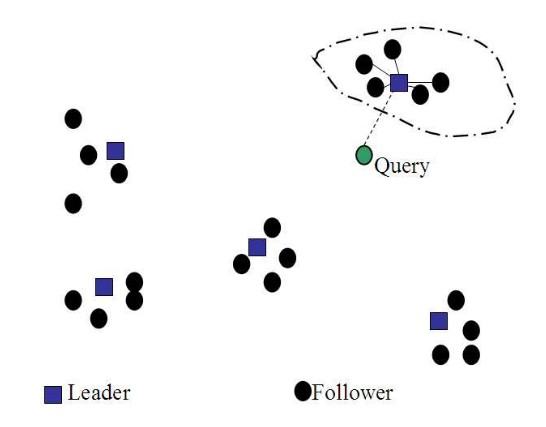
\includegraphics[scale=0.60]{sect7/figure_7_3.png}
    \caption{Cluster pruning.}
\end{figure}

\subsection{Components of an information retrieval system}
In this section we combine the ideas developed so far to describe a rudimentary search system that retrieves and scores documents.

\paragraph{Tiered indexes}
Heuristics such as index elimination for inexact top-$K$ retrieval, we may occasionally find ourselves with a set $A$ of contenders that has fewer than $K$ documents. A common solution to this issue is the user of \textbf{tiered indexes}. In this example we set a tf threshold of 20 for tier 1 and 10 for tier 2, meaning that the tier 1 index only has postings entries with tf values exceeding 20, while the tier 2 index only has postings entries with tf values exceeding 10.

\paragraph{Query-term proximity}
Especially for free text queries, users prefer a document in which most or all of the query terms appear close to each other. Consider a query with two or more query terms, $t_1, t_2, \dots , t_k$. Let $\omega$ be the width of the smallest window in a document $d$ that contains all the query terms, measured in the number of words in the window. For instance, \code{The quality of mercy is not strained}, the smallest window for the query \code{strained mercy} would be 4. The smaller that $\omega$ is, the better that $d$ matches the query. In cases where the document does not contain all of the query terms, we can set $\omega$ to be some enormous number. Such proximity-weighted scoring functions are a departure from pure cosine similarity and closer to the \textit{soft conjunctive} semantics.

How can we design such a proximity-weighted scoring function to depend on $\omega$? The simplest answer relies on a \textit{hand coding} technique. In a more scalable approach, we treat the integer $\omega$ as yet another feature in the scoring function, whose importance is assigned by machine learning.

\paragraph{Designing parsing and scoring functions}
Common search interfaces tend to mask query operators from the end user. The intent is to hide the complexity of these operators from the largely non-technical audience, inviting \textbf{free text queries}. How should a search equipped with indexes for various retrieval operators treat a query such as \code{rising interest rates}? Typically, a \textbf{query}
\begin{figure}[H]
    \centering
    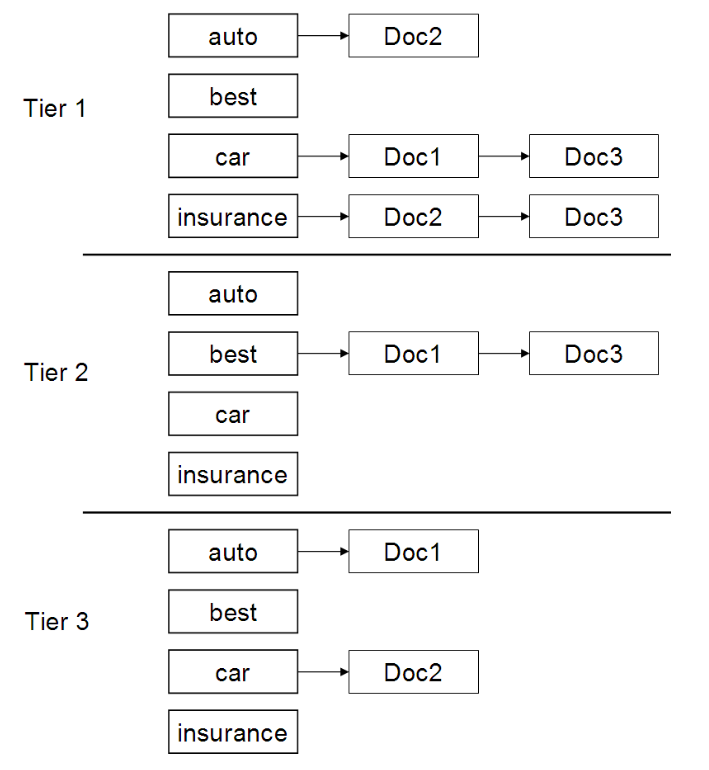
\includegraphics[scale=0.60]{sect7/figure_7_4.png}
    \caption{Tiered indexes. If we fail to get $K$ results from tier 1, query processing
“falls back” to tier 2, and so on. Within each tier, postings are ordered by document ID.}
\end{figure}
\noindent
\textbf{parser} is used to translate the user-specified keywords into a query with various operators that is executed against the underlying indexes. Sometimes, this execution can entail multiple queries against the underlying indexes; for example, the query parser may issue a stream of queries:
\begin{enumerate}
    \item Run the user-generated query string as a phrase query. Rank them by vector space scoring using as query the vector consisting of the 3 terms \code{rising interest rates}.
    \item If fewer than ten documents contain the phrase \code{rising interest rates}, run the two 2-term phrase queries \code{rising interest} and \code{interest rates}; rank these using vector space scoring.
    \item If we still have fewer than ten results, run the vector space query consisting of the three individual query terms.
\end{enumerate}
Each of these steps may yield a list of scored documents, for each of which we compute a score. This score must combine contributions from vector space scoring, static quality, proximity weighting and potentially other factors. This demands an aggregate scoring function that \textbf{accumulates evidence} of a document’s relevance from multiple sources. 

\paragraph{Putting it all together}
In \ref{Complete-scheme}, documents stream in from the left for parsing and linguistic processing (language and format detection, tokenization and stemming). The resulting stream of tokens feeds into two modules. First, we retain a copy of each parsed document in a document cache. A second copy of the tokens is fed to a bank of indexers that create a bank of indexes including zone and field indexes that store the metadata for each document, (tiered) positional indexes, indexes for spelling correction and other tolerant retrieval, and structures for accelerating inexact top-$K$ retrieval. A free text user query (top center) is sent down to the indexes both directly and through a module for generating spelling-correction candidates. Retrieved documents (dark arrow) are passed to a scoring module that computes scores based on machine-learned ranking (MLR). Finally, these ranked documents are rendered as a results page.
\begin{figure}[H]
    \centering
    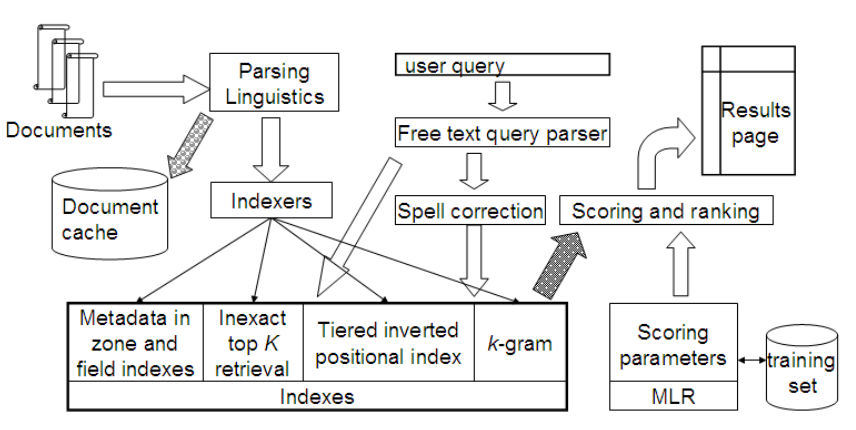
\includegraphics[scale=0.65]{sect7/figure_7_5.png}
    \caption{A complete search system. Data paths are shown primarily for a free text query.}
    \label{Complete-scheme}
\end{figure}

\subsection{Vector space scoring and query operator interaction}

Vector space scoring supports so-called free text retrieval, in which a query is specified as a set of words without any query operators connecting them. It allows documents matching the query to be scored and thus ranked, unlike the Boolean, wildcard and phrase queries. The interpretation of such free text queries was that at least one of the query terms be present in any retrieved document. However more recently, web search engines such as Google have popularized the notion that a set of terms typed into their query boxes carries the semantics of a conjunctive query that only retrieves documents containing all or most query terms.

\section{Evaluation in information retrieval}
\subsection{Information retrieval system evaluation}
To measure ad hoc information retrieval effectiveness in the standard way, we need a test collection consisting of three things:
\begin{enumerate}
    \item A document collection
    \item A test suite of information needs, expressible as queries
    \item A set of relevance judgments, standardly a binary assessment of either \textit{relevant} or \textit{nonrelevant} for each query-document pair.
\end{enumerate}
The standard approach to information retrieval system evaluation revolves around the notion of \textbf{relevant} and \textbf{nonrelevant} documents. With respect to a
user information need, a document in the test collection is given a \textbf{binary classification} as either relevant or nonrelevant. This decision is referred to as the \textbf{ground truth} judgment of relevance. The test document collection needs have to be of a reasonable size: 50 information needs has usually been found to be a sufficient minimum.

Relevance is assessed relative to an information need, not a query. For example, an information need might be:
\medskip\\
\indent Information on whether drinking red wine is more effective at reducing your risk of heart attacks than white wine.
\medskip\\
This might be translated into a query such as:
\medskip\\
\indent wine \code{AND} red \code{AND} white \code{AND} heart \code{AND} attack \code{AND} effective
\medskip\\
A document is relevant if it addresses the stated information need, not because it just happens to contain all the words in the query. To evaluate a system, we require an expression of an information need, which can be used for judging returned documents.

Many systems contain various weights (parameters) that can be adjusted to tune system performance. It is wrong to report results on a test collection which were obtained by tuning these parameters to maximize performance on that collection. The correct procedure is to have one or more \textbf{development test collections}, and to tune the parameters on the development test collection.

\subsection{Standard test collections}
Here is a list of the most standard test collections and evaluation series.
\begin{itemize}
    \item The \textit{Cranfield} collection.
    \item \textit{Text Retrieval Conference} (TREC).
    \item \textit{NII Test Collections for IR Systems} (NTCIR).
    \item \textit{Cross Language Evaluation Forum} (CLEF).
    \item \textit{Reuters-21578} and \textit{Reuters-RCV1}.
    \item \textit{20 Newsgroups}.
\end{itemize}

\subsection{Evaluation of unranked retrieval sets}
The two most frequent and basic measures for information retrieval effectiveness are precision and recall.

\textbf{Precision} (P) is the fraction of retrieved documents that are relevant
\[
\textrm{Precision} = \frac{\textrm{\#(relevant items retrieved)}}{\textrm{\#(retrieved items)}} = P(\textrm{relevant|retrieved})
\]

\textbf{Recall} (R) is the fraction of relevant documents that are retrieved
\[
\textrm{Recall} = \frac{\textrm{\#(relevant items retrieved)}}{\textrm{\#(relevant items)}} = P(\textrm{retrieved|relevant})
\]
These notions can be summerized in the following table:
\begin{table}[H]
\centering
\begin{tabular}{|l|l|l|}
\hline
              & Relevant             & Nonrelevant          \\ \hline
Retrieved     & true positives (tp)  & false positives (fp) \\ \hline
Non retrieved & false negatives (fn) & true negatives (tn)  \\ \hline
\end{tabular}
\end{table}
Then:
\begin{equation}
\begin{split}
    P = tp / (tp + fp) \\
    R = tp / (tp + fn)    
\end{split}
\end{equation}

An alternative is \textbf{accuracy}, the fraction of the classifications that are correct: 
\[
accuracy = (tp + tn)/(tp + fp + fn + tn).
\]
There is a good reason why accuracy is not an appropriate measure for information retrieval problems. In almost all circumstances, the data is extremely skewed: normally over 99.9\% of the documents are in the nonrelevant category. A system tuned to maximize accuracy can appear to perform well by simply deeming all documents nonrelevant to all queries. Even if the system is quite good, trying to label some documents as relevant will almost always lead to a high rate of false positives. The measures of precision and recall concentrate the evaluation on the return of true positives, asking what percentage of the relevant documents have been found and how many false positives have also been returned.

The advantage of having the two numbers for precision and recall is that one is more important than the other in many circumstances. For example, web surfers would like every result on the first page to be relevant (high precision). The two quantities trade off against one another: you can always get a recall of 1 (but very low precision) by retrieving all documents for all queries. On the other hand, in a good system, precision usually decreases as the number of documents retrieved is increased. In general we want to get some amount of recall while tolerating only a certain percentage of false positives.

A single measure that trades off precision versus recall is the \textbf{F measure}, which is the weighted harmonic mean of precision and recall:
\[
\textrm{F} = \frac{1}{\alpha \frac{1}{P} + (1 - \alpha) \frac{1}{R}} = \frac{(\beta^2 + 1)PR}{\beta^2P + R} \quad \textrm{where} \quad \beta^2 = \frac{1 - \alpha}{\alpha}
\]
where $\alpha \in [0,1]$ and thus $\beta \in [0, \infty]$. The default\textbf{ balanced F measure} equally weights precision and recall, which means making $\alpha = 1/2$ or $\beta = 1$. It is commonly written as $F_1$. When using $\beta = 1$, the formula simplifies to:
\[
F_{\beta=1} = \frac{2PR}{P + R}
\]
Values of $\beta < 1$ emphasize precision, while values of $\beta > 1$ emphasize recall.

\subsection{Evaluation of ranked retrieval results}
Precision, recall, and the F measure are set-based measures. They are computed using unordered sets of documents. We need to extend these measures if we are to evaluate the ranked retrieval results. In a ranked retrieval context, appropriate sets of retrieved documents are naturally given by the top $k$ retrieved documents. For each such set, precision and recall values can be plotted to give a \textbf{precision-recall curve}:
if the $(k + 1)^{th}$ document retrieved is nonrelevant then recall is the same as for the top k documents, but precision has dropped. If it is relevant, then both precision and recall increase, and the curve jags up and to the right.
\begin{figure}[H]
    \centering
    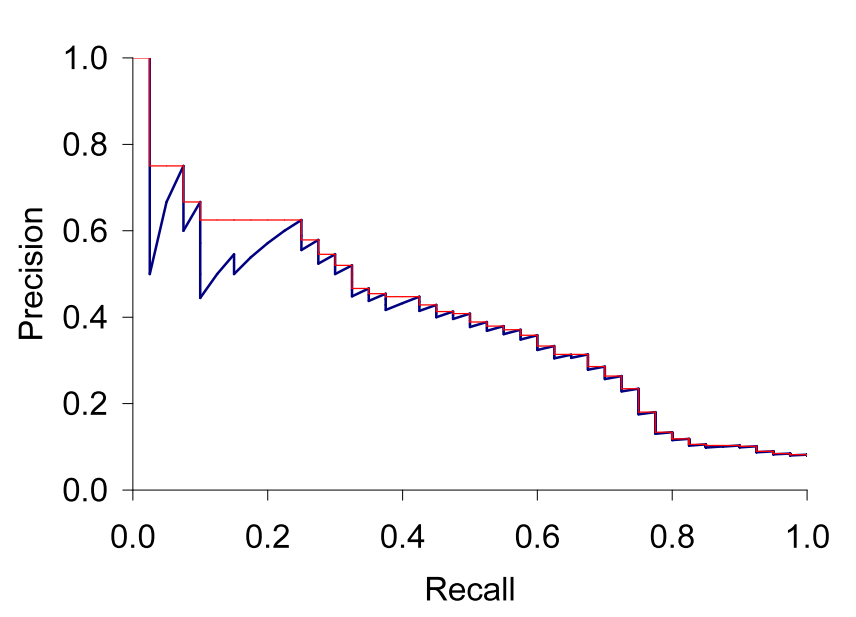
\includegraphics[scale=0.55]{sect8/figure_8_2.png}
    \caption{Precision/recall graph}
\end{figure}
It is often useful to remove these jiggles and the standard way to do this is with an interpolated precision: the \textbf{interpolated precision} $p_{interp}$ at a certain recall level $r$ is defined as the highest precision found for any recall level $r' \geq r$:
\[
p_{interp}(r) = \max_{r' \geq r}p(r') 
\]
The justification is that almost anyone would be prepared to look at a few more documents if it would increase the percentage of the viewed set that were relevant.

Examining the entire precision-recall curve is very informative, but there is often a desire to reduce this information down to a few numbers. The traditional way of doing this is the \textbf{11-point interpolated average precision}. For each information need, the interpolated precision is measured at the 11 recall levels of 0.0, 0.1, 0.2,..., 1.0. For each recall level, we then calculate the arithmetic mean of the interpolated precision at that recall level for each information need in the test collection.

Other measures have become more common. Most standard among the TREC community is \textbf{Mean Average Precision} (\textbf{MAP}). For a single information need, Average Precision is the average of the precision value obtained for the set of top $k$ documents existing after each relevant document is retrieved. If the set of relevant documents for an information need $q_j \in Q \textrm{is} {d_1,\dots,d_{mj}}$ and $R_{jk}$ is the set of ranked retrieval results from the top result until you get to document $d_k$, then
\[
\textrm{MAP($Q$)} = \frac{1}{|Q|} \sum_{j = 1}^{|Q|}{\frac{1}{m_j}} \sum_{k = 1}^{m_j}{\textrm{Precision}(R_{jk})}
\]
When a relevant document is not retrieved at all, the precision value in the above equation is taken to be 0.
Using MAP, fixed recall levels are not chosen, and there is no interpolation. 
\begin{figure}[H]
    \centering
    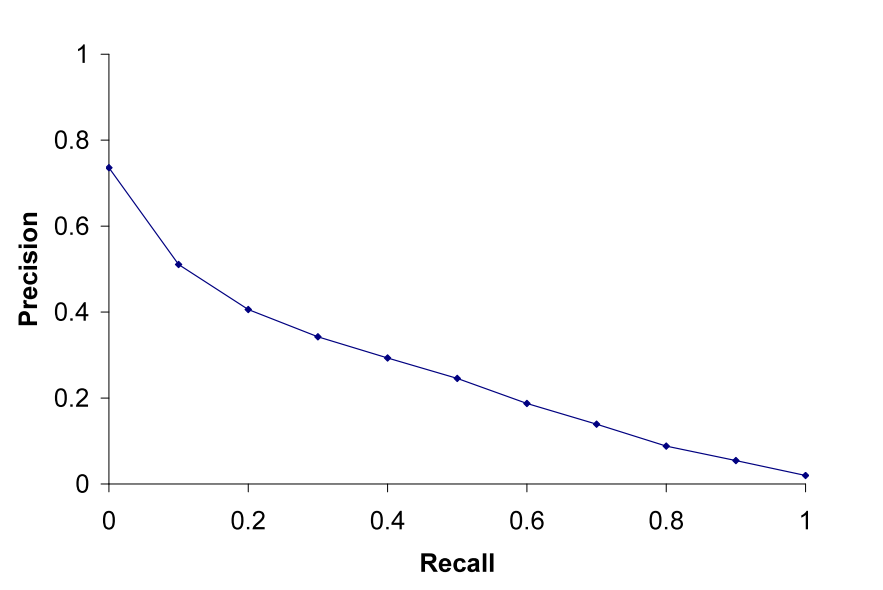
\includegraphics[scale=0.55]{sect8/figure_8_3.png}
    \caption{Averaged 11-point precision/recall graph across 50 queries for a representative TREC system. The Mean Average Precision for this system is 0.2553.}
\end{figure}

The above measures factor in precision at all recall levels. For many prominent applications, particularly web search, this may not be relevant to users. What matters is rather how many good results there are on the first page or the first three pages. This leads to measuring precision at fixed low levels of retrieved results, such as 10 or 30 documents. This is referred to as \textbf{Precision at $k$}. It has the advantage of not requiring any estimate of the size of the set of relevant documents but the disadvantages that it is the least stable of the commonly used evaluation measures.

An alternative, is \textbf{$R$-precision}. It requires having a set of known relevant documents $Rel$, from which we calculate the precision of the top $Rel$ documents returned. $R$-precision adjusts for the size of the set of relevant documents. A perfect system could score 1 on this metric for each query, whereas, even a perfect system could only achieve a precision at 20 of 0.4 if there were only 8 documents in the collection relevant to an information need. If there are $|Rel|$ relevant documents for a query, we examine the top $|Rel|$ results of a system, and find that $r$ are relevant, then by definition, not only is the precision $r/|Rel|$, but the recall of this result set is also $r/|Rel|$. Like Precision at $k$, $R$-precision describes only one point on the precision-recall curve. $R$-precision turns out to be highly correlated with MAP empirically.

Another concept sometimes used in evaluation is an \textbf{ROC curve} (Receiver Operating Characteristics). An ROC curve plots the true positive rate or sensitivity (recall) against the false positive rate or (1 − specificity). The false positive rate is given by $fp / (fp + tn)$.
\begin{figure}[H]
    \centering
    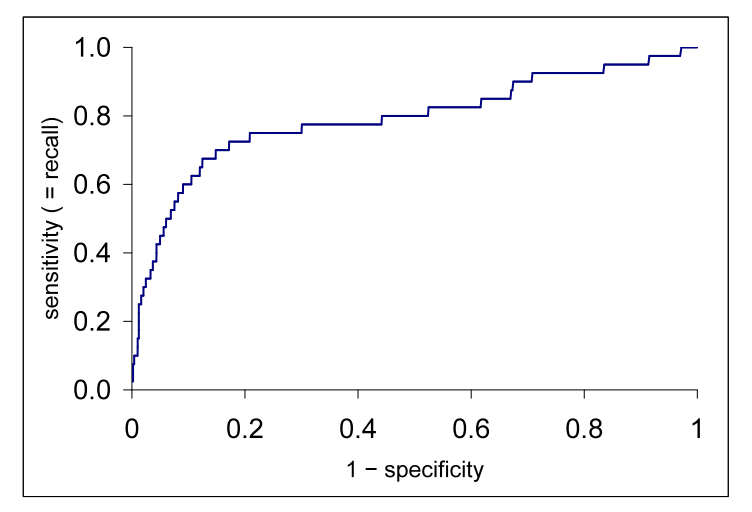
\includegraphics[scale=0.55]{sect8/figure_8_4.png}
    \caption{The ROC curve corresponding to the precision-recall curve in Figure 32.}
\end{figure}

A final approach is measures of \textbf{cumulative gain}, and in particular \textbf{normalized discounted cumulative gain} (NDCG). NDCG is designed for situations of non-binary notions of relevance. Like precision at $k$, it is evaluated over some number $k$ of top search results. % For a set of queries $Q$, let $R(j, d)$ be the relevance score assessors gave to document $d$ for query $j$. Then,

\subsection{Assessing relevance}
To properly evaluate a system, your test information needs must be germane to the documents in the test document collection, and appropriate for predicted usage of the system. Given information needs and documents, you need to collect relevance assessments. This is a time-consuming and expensive process involving human beings. For large modern collections, it is usual for relevance to be assessed only for a subset of the documents for each query. The most standard approach is \textbf{pooling}, where relevance is assessed over a subset of the collection that is formed from the top $k$ documents returned by a number of different IR systems.

A human is not a device that reliably reports a gold standard judgment of relevance, humans and their relevance judgments are quite idiosyncratic and variable. The success of an IR system depends on how good it is at satisfying the needs of humans.

In the social sciences, a common measure for agreement between judges is the \textbf{kappa statistic}. It is designed for categorical judgments and corrects a simple agreement rate for the rate of chance agreement.
\[
kappa = \frac{P(A) - P(E)}{1 - P(E)}
\]
where $P(A)$ is the proportion of the times the judges agreed, and $P(E)$ is the proportion of the times they would be expected to agree by chance. The kappa value will be 1 if two judges always agree, 0 if they agree only at the rate given by chance, and negative if they are worse than random. If there are more than two judges, it is normal to calculate an average pairwise kappa value.

\paragraph{Critiques and justifications of the concept of relevance}
Once we have a formal measure that we have confidence in, we can proceed to optimize effectiveness by machine learning methods.

Assessments are binary. Relevance of a document to an information need is treated as an absolute, objective decision. But judgments of relevance are subjective, varying across people. Human assessors are also imperfect measuring instruments, susceptible to failures of understanding and attention. We also have to assume that users’ information needs do not change as they start looking at retrieval results. Any results based on one collection are heavily skewed by the choice of collection, queries, and relevance judgment set: the results may not translate from one domain to another or to a different user population.

One clear problem with the relevance-based assessment is the distinction between relevance and \textbf{marginal relevance}: whether a document still has distinctive usefulness after the user has looked at certain other documents. Even if a document is highly relevant, its information can be completely redundant with other documents which have already been examined. Maximizing marginal relevance requires returning documents that exhibit diversity and novelty.

\section{Relevance feedback and query expansion}









%++++++++++++++++++++++++++++++++++++++++
% References section will be created automatically 
% with inclusion of "thebibliography" environment
% as it shown below. See text starting with line
% \begin{thebibliography}{99}
% Note: with this approach it is YOUR responsibility to put them in order
% of appearance.

%\newpage
%\begin{thebibliography}{99}
%\end{thebibliography}

\end{document}
